\documentclass[9pt,a4paper]{beamer}
%\usepackage[utf8]{inputenc}
\usepackage[output-decimal-marker={.}]{siunitx}
\usepackage[compat=1.1.0]{tikz-feynman}
\usepackage{amsmath}
\usepackage[most]{tcolorbox}
\usepackage{bm}
\tikzfeynmanset{every blob = {minimum size = 2mm}}

\newcommand{\commento}[1]{}
\setbeamercolor{block title}{fg=white, bg=orange}

\beamertemplatenavigationsymbolsempty

%TITOLO TESI
%\usetheme{Madrid}
\usetheme{CambridgeUS}
\author[Adriano Del Vincio]{Adriano Del Vincio 562946\\ \footnotesize Relatori: prof. Francesco Forti, Prof. Concettina Sfienti}
\institute[Università di Pisa]{\textbf {Università di Pisa}}
\title[Tesi di Laurea]{Commissioning and First Data Analysis of the Mainz Radius Experiment}
\subtitle{}
\date{20/07/2023}
\titlegraphic{
\includegraphics[width=0.3\textwidth]{MarchioUnipi.pdf}}
\setbeamerfont{title}{shape=\itshape,family=\rmfamily}

\begin{document}
%\setlength{\belowdisplayskip}{3pt}
%\setlength{\abovedisplayskip}{3pt}


%TITOLO 
\frame{\titlepage}


% 1 INTRODUZIONE MREX 
\begin{frame}{The Mainz Radius Experiment}
\framesubtitle{MREX}

The Mainz Radius Experiment is an experimental campaign at the nuclear physics institute of Mainz, with the aim of investigating the properties of nuclear matter with imbalance in the number of protons and neutrons.

\begin{block}{Objective}
Determination of the neutron spacial density for $^{208}Pb$ nucleus, through the elastic electron scattering. From an accurate determination of the neutron spacial distribution, the \textit{Neutron Skin Thickness} of $^{208}Pb$ is measured.
\end{block}

\begin{columns}[T]
\begin{column}{.7\textwidth}
The neutron skin thickness is defined as the difference between rms radius of neutron and proton spacial distributions:
\begin{equation}
\delta r_{np} = \sqrt{\vphantom{r^{2}_{p}}<r^{2}_{n}>} - \sqrt{<r^{2}_{p}>} ,
\end{equation}
\end{column}
\begin{column}{.3\textwidth}
\centering
\includegraphics[width = 0.75\textwidth]{figures/lead.pdf}
\end{column}
\end{columns}
\end{frame}

% 2 MREX e Neutron Skin
\begin{frame}{MREX and Neutron Skin Thickness}

The results of the experiment will be valuable to constrain the Equation of State (\textbf{EOS}) of nuclear matter. The EOS of nuclear matter plays an important role for the \textbf{neutron star structure}, specifically the determination of the radius $R_{ns}$. \smallskip

\begin{columns}[T]
\begin{column}{.5\textwidth}
\commento{The neutron skin thickness is determined by the competition of two terms of the nuclear binding energy: the surface term and the symmetry energy.}
In neutron rich nuclei, the spacial distribution of neutrons in \textbf{more extended} than proton one.
Theoretical models link the Neutron skin thickness of heavy nuclei, such as $^{208}Pb$, with the slope of the symmetry energy \textbf{L}.

\end{column}
\begin{column}{.5\textwidth}
\begin{figure}
\centering
\includegraphics[width = 1\textwidth]{figures/SpacialDistribution.png}
\caption{Neutron (black line) and proton (red line) spacial distributions as predicted by FSUGold model. The blue dots represents the experimental data of $^{208}Pb$ charge density.}
\end{figure}
\end{column}
\end{columns}
\end{frame}

% 3 SLOPE OF THE SYMMETRY ENERGY
\begin{frame}{Symmetry Energy}{Neutron Skin and Symmetry Energy}

\begin{equation}
\begin{split}
\epsilon(\rho, \alpha) &= \epsilon_{SNM}(\rho) + \alpha^{2} S(\rho) + O(\alpha^{4}) \\
S(\rho) &= J + L \cdot (\dfrac{\rho - \rho_{0}}{3 \rho_{0}}) + ...
\end{split}
\end{equation} 

\begin{columns}[T]
\begin{column}{0.5\textwidth}
\begin{center}
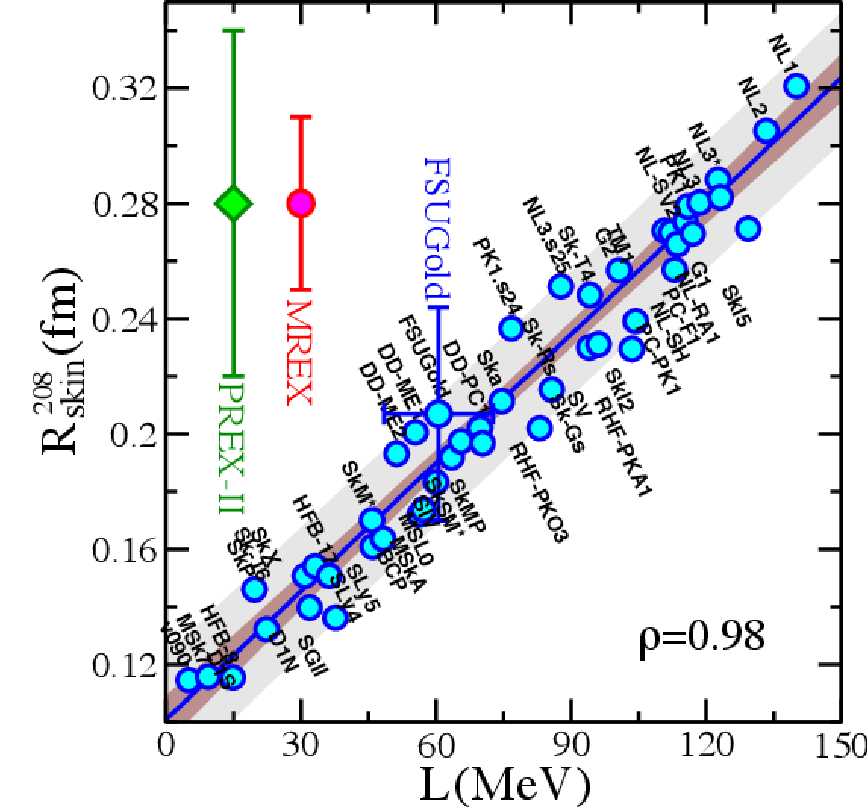
\includegraphics[width = 0.95\textwidth]{figures/LvsR1.pdf}
\end{center}
\end{column}
\begin{column}{0.5\textwidth}
 \medskip The symmetry energy $S(\rho)$ is the key component of the equation of state which controls the neutron skin thickness. $S(\rho)$ quantifies the change in energy related to the neutron-proton asymmetry. 
\end{column}
\end{columns}


\end{frame}

% 4 Neutron Skin and Neutron Star Radius
\begin{frame}{Neutron Skin and Neutron Star Radius}
\begin{columns}[T]
\begin{column}{.5\textwidth}
The slope of the symmetry energy is related to both the \textbf{neutron skin} of lead and \textbf{neutron star radius}. The radius of the neutron star is determined from Tolman-Oppenheimer-Volkoff (TOV) equation.
 Giving the pressure $P_{c}$ at the center of the star, the radius $R$ can be determined. But for neutron star, the pressure at the center is strongly related to the \textbf{pressure of pure neutron matter}, in large part determined by $L$.
 
 \begin{equation}
 P = \frac{1}{3} \rho_{0} L
 \end{equation}
\end{column}
\begin{column}{.5\textwidth}
\begin{figure}
\centering
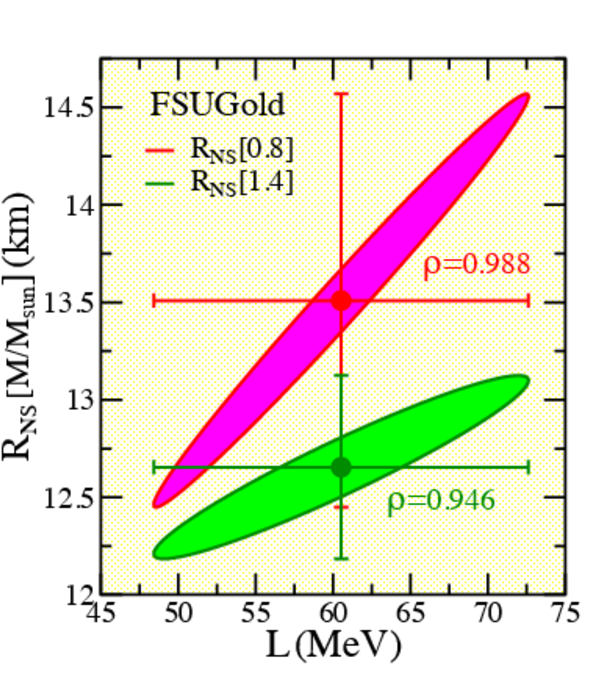
\includegraphics[scale=0.50]{figures/LvsRns.pdf}
\caption{Covariance ellipses displaying the correlation between the neutron star radius and the slope of the symmetry energy, as predicted by FSUGold model.}
\end{figure}
\end{column}
\end{columns}
\end{frame}

% 6 PARITY VIOLATING ASYMMETRY
\begin{frame}
\frametitle{Parity Violating Asymmetry}
\framesubtitle{Measurement of the Neutron Spacial Distribution of Lead}

The determination of the neutron spacial distribution relies on the electron-nucleus elastic scattering. 
The neutron spacial distribution is measured via the parity violating scattering, where longitudinal polarized electrons scatter from a fixed lead target. The experiment is planned at the future MESA accelerator. 

\begin{equation}
A_{pv} = \dfrac{\sigma_{R} - \sigma_{L}}{\sigma_{R} + \sigma_{L}}
\end{equation}

The key quantity is the asymmetry in the cross-section due to the different polarization state of the beam.
\begin{columns}[]
\begin{column}{0.75\textwidth}
\vspace{-15pt}
\begin{figure}[!ht]
\[
\feynmandiagram [scale =  0.8, transform shape][vertical = c to d]{
	a [particle = \(e^{-}\)] -- [fermion, thick] c -- [fermion, thick] g [particle = \(e^{-}\)],
	c -- [photon, edge label' = \(\gamma\), momentum = {[arrow style = blue]\(k\)}] d [blob],
	h [particle = \(^{208}Pb\)] -- [fermion, thick] d -- [fermion, thick] j [particle = \(^{208}Pb\)],
	};
\qquad \qquad
\feynmandiagram [scale = 0.8, transform shape][vertical = c to d]{
	a [particle = \(e^{-}\)] -- [fermion, thick] c -- [fermion, thick] g [particle = \(e^{-}\)],
	c -- [photon, edge label' = \(Z\), momentum = {[arrow style = blue]\(k\)}] d [blob],
	h [particle = \(^{208}Pb\)] -- [fermion, thick] d -- [fermion, thick] j [particle = \(^{208}Pb\)],
	};
\]
\end{figure}
\end{column}
\begin{column}{0.25\textwidth}
\begin{itemize}
\item $Q_{p} = 0.04$
\item $Q_{n} = -0.99$
\end{itemize}
\end{column}
\end{columns}
\end{frame}

% 7 INTRODUZIONE ALLA TRANSVERSE ASYMMETRY
\begin{frame}{Transverse Asymmetry}
 
The transverse asymmetry, or Beam Normal Single Spin Asymmetry, is the cross-section asymmetry for electrons polarized in the normal plane ($\frac{\vec{k'} \wedge \vec{k}}{ |\vec{k}| |\vec{k'}|}$) : 

\begin{equation*}
A_{transverse} = \dfrac{\sigma_{\uparrow} -  \sigma_{\downarrow}}{\sigma_{\uparrow} + \sigma_{\downarrow}}
\end{equation*}

The asymmetry arises from the interference of:

\begin{columns}
\begin{column}{0.5\textwidth}
\begin{figure}[hbtp]
\[
\feynmandiagram [scale = 0.8, transform shape][vertical = c to d]{
	a [particle = \(e^{-}\)] -- [fermion, thick] c -- [fermion, thick] g [particle = \(e^{-}\)],
	c -- [photon, edge label' = \(\gamma\), momentum = {[arrow style = blue]\(k\)}] d [blob],
	h [particle = \(^{208}Pb\)] -- [fermion, thick] d -- [fermion, thick] j [particle = \(^{208}Pb\)],
	};
\qquad 
\feynmandiagram [scale = 0.8, transform shape][baseline = (h), horizontal = d to j]{
	a [particle = \(e^{-}\)] -- [fermion, thick] c -- [fermion, thick, edge label' = \(e\), momentum = {[arrow style = blue]\(k_{1}\)}] f -- [fermion, thick] g [particle = \(e^{-}\)],
	c -- [photon, edge label = \(\gamma\)] d [blob],
	f -- [photon, edge label = \(\gamma\)] j [blob],
	h [particle = \(^{208}Pb\)]-- d -- [fermion, thick] j -- k [particle = \(^{208}Pb\)] ,
	};
\]
\end{figure}
\end{column}
\begin{column}{0.5\textwidth}
\begin{figure}
\centering
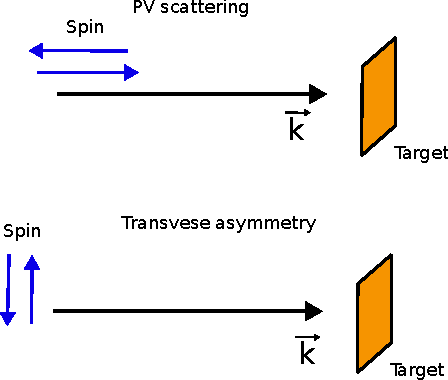
\includegraphics[width = 0.70\textwidth]{PvTa.pdf}
\end{figure}
\end{column}
\end{columns}
\end{frame}

% 8 TRANSVERSE ASYMMETRY
\begin{frame}{Transverse Asymmetry}

The incident beam is made by $\SI{570}{\mega \electronvolt}$ electrons, that are polarized along the transverse axes ($\uparrow$ and $\downarrow$). The physical quantity to measure is the asymmetry between the number of scattered electrons, due to the change of the polarity:

\begin{equation}
asym = \frac{N_{+} - N_{-}}{N_{+} + N_{-}} \text{(expected $\sim$ +/- 20 ppm, Q = \SI{0.2}{\giga\electronvolt c^{-1}})}
\end{equation}

\begin{columns}[T]
\begin{column}{.5\textwidth}

The prediction for the transverse asymmetry is given by the formula below:

\begin{equation}
A_{n} \simeq C_{0} \log \frac{Q^{2}}{m^2_e c^2} \frac{F_{Compton} (Q^2)}{F_{ch}(Q^2)}
\end{equation}
\end{column}
\begin{column}{.5\textwidth}
\centering
\begin{figure}
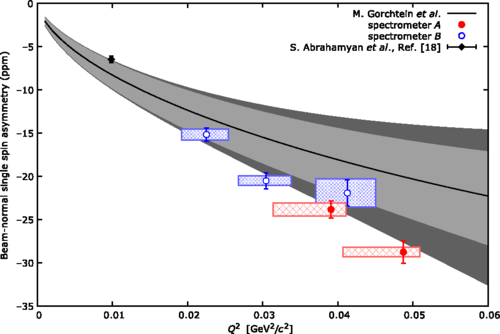
\includegraphics[width = \textwidth]{figures/medium.png}
\caption{Asymmetry versus transferred momentum for selected nuclei.}
\end{figure}
\end{column}
\end{columns}

\end{frame}

% 9 SCHEMA MREX
\begin{frame}[t]{MREX SCHEME}
\begin{columns}[T]
\begin{column}{0.40\textwidth}
Scheme of the experimental campaign of MREX. The work of the thesis correspond to the first step of the diagram, the commissioning of the new setup for the measurement of the transverse asymmetry on $^{12}C$.
\end{column}
\begin{column}{0.60\textwidth}
\begin{figure}
\centering
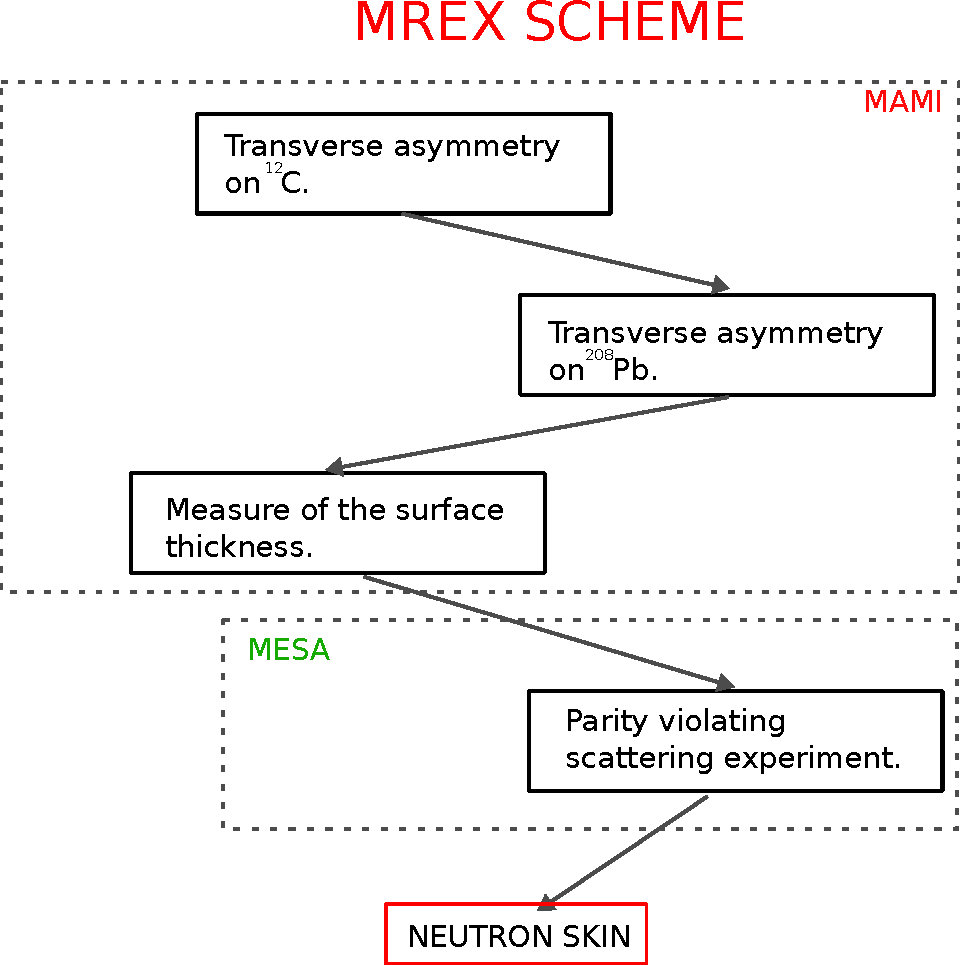
\includegraphics[width = 0.85\textwidth]{SchemeMrex.pdf}
\caption{\footnotesize Scheme of MREX.}
\end{figure}
\end{column}
\end{columns}
\end{frame}


\begin{frame}[noframenumbering]{MAMI}
\begin{center}
\color{red}{\Large \bf{MAMI ELECTRON ACCELERATOR}}
\end{center}
\end{frame}

% 11 MAMI ACCELERATORE
\begin{frame}{MAMI Electron Accelerator}

\begin{figure}[hbtp]
\centering
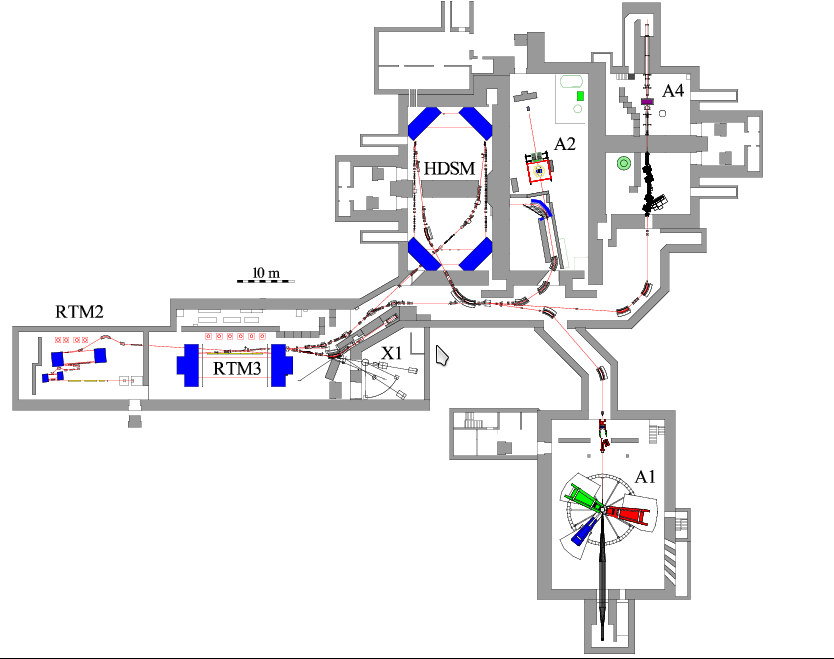
\includegraphics[width = 0.65\textwidth]{figures/mami.png}
\caption{ \footnotesize Scheme of MAMI accelerator. RTM2 is the first acceleration stage, where the electrons are extracted from the source. RTM3 corresponds to the final acceleration stage of the experiment (\SI{570}{\mega \electronvolt}), A1 is the experiment hall where the experiment described is the thesis is set up.}
\end{figure}

\end{frame}

\begin{frame}{Race Track Microtron Scheme}

\begin{figure}[hbtp]
\centering
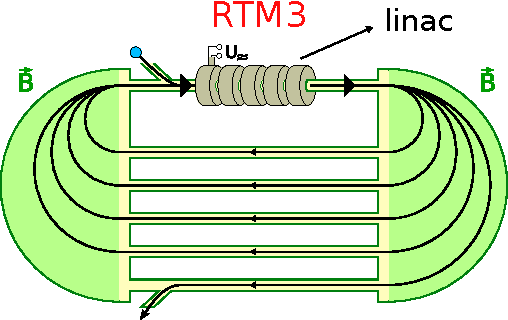
\includegraphics[width = 0.95\textwidth]{figures/RacetrackMicrotronSketch.pdf}
\end{figure}

\end{frame}

\begin{frame}{RTM3}{Race Track Microtron 3 of MAMI}

\begin{figure}[hbtp]
\centering
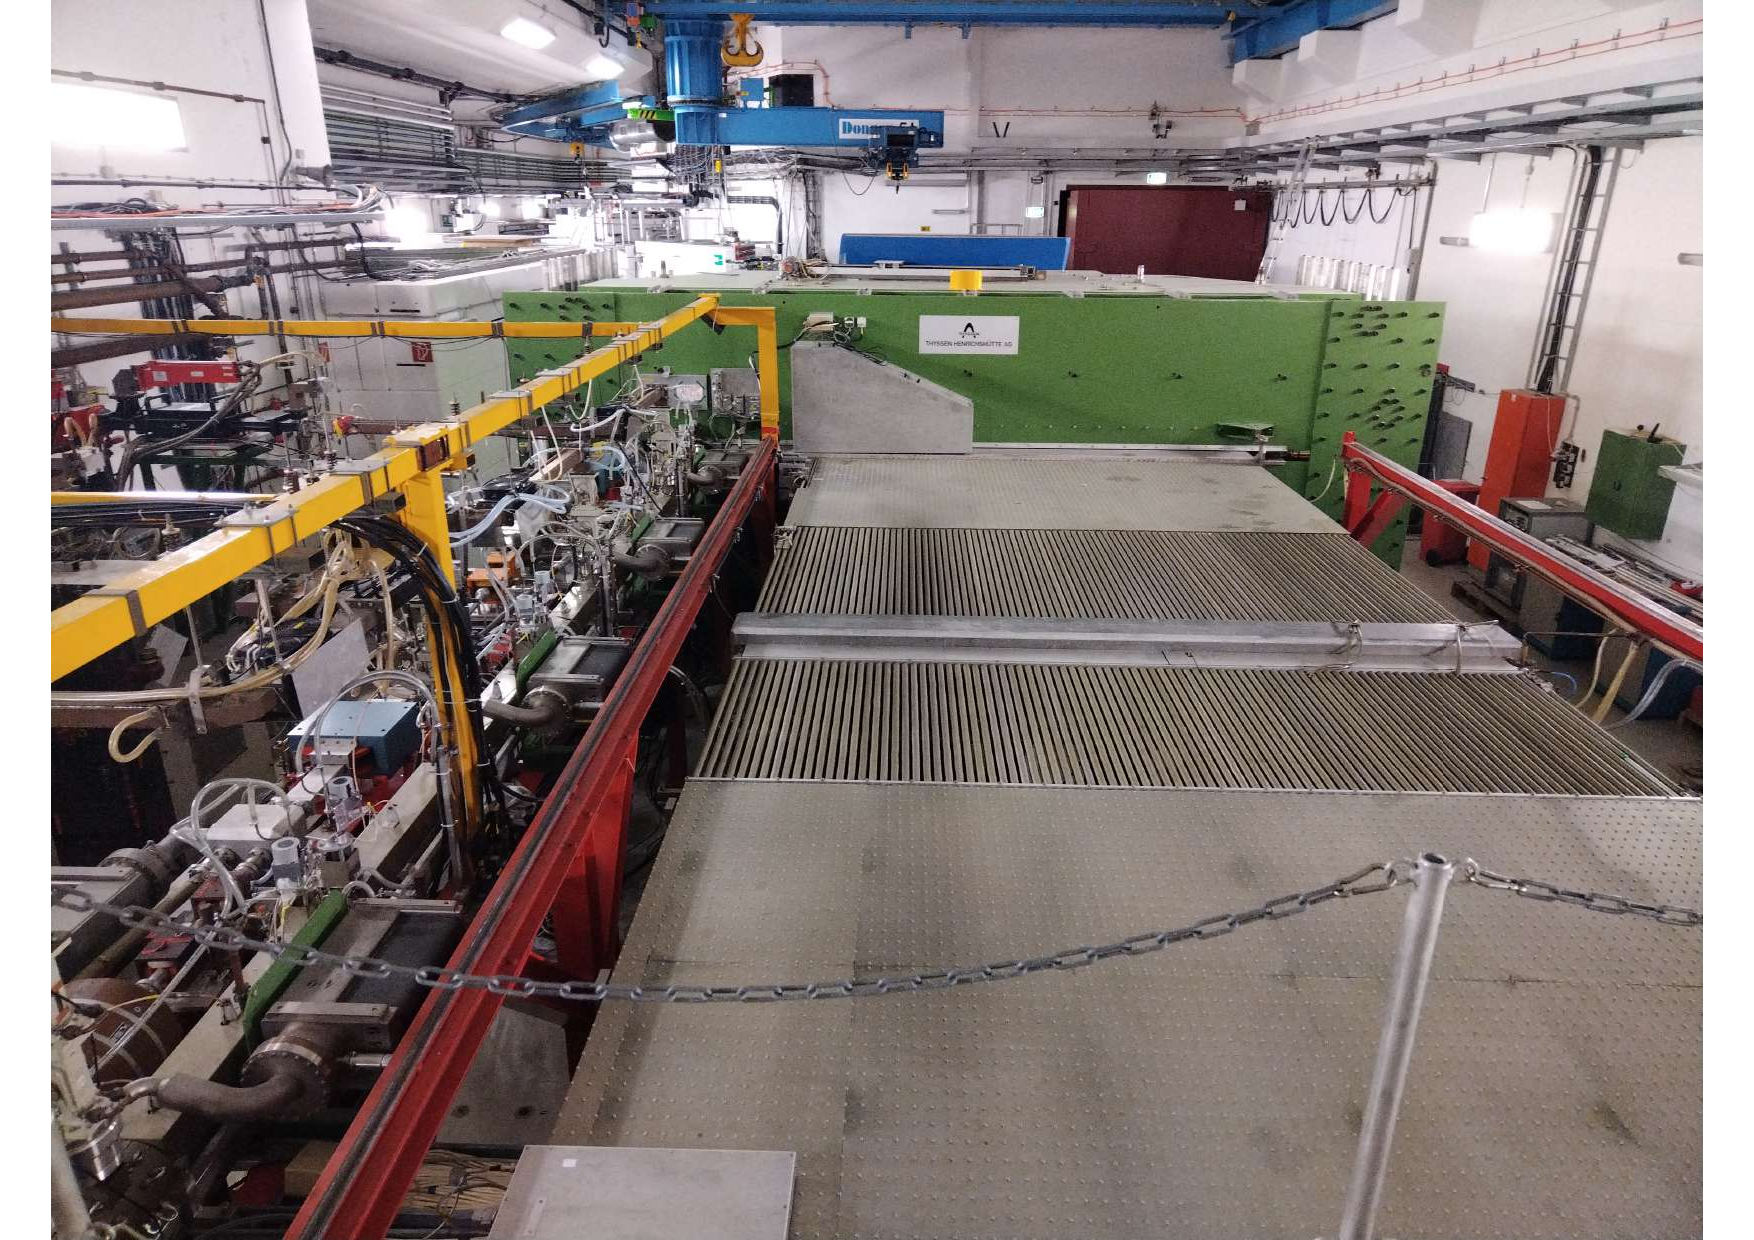
\includegraphics[width = 0.80\textwidth]{figures/Racetrack.pdf}
\end{figure}

\end{frame}

% 12 Sala Sperimentale
\begin{frame}{A1 Experimental Hall}{MAMI Electron Accelerator}

\begin{columns}[T]
\begin{column}{.5\textwidth}
In MAMI A1, three large spectrometers are positioned on a rail track around the scattering chamber. For the experiment, only the red and blue spectrometers were used.
\begin{center}
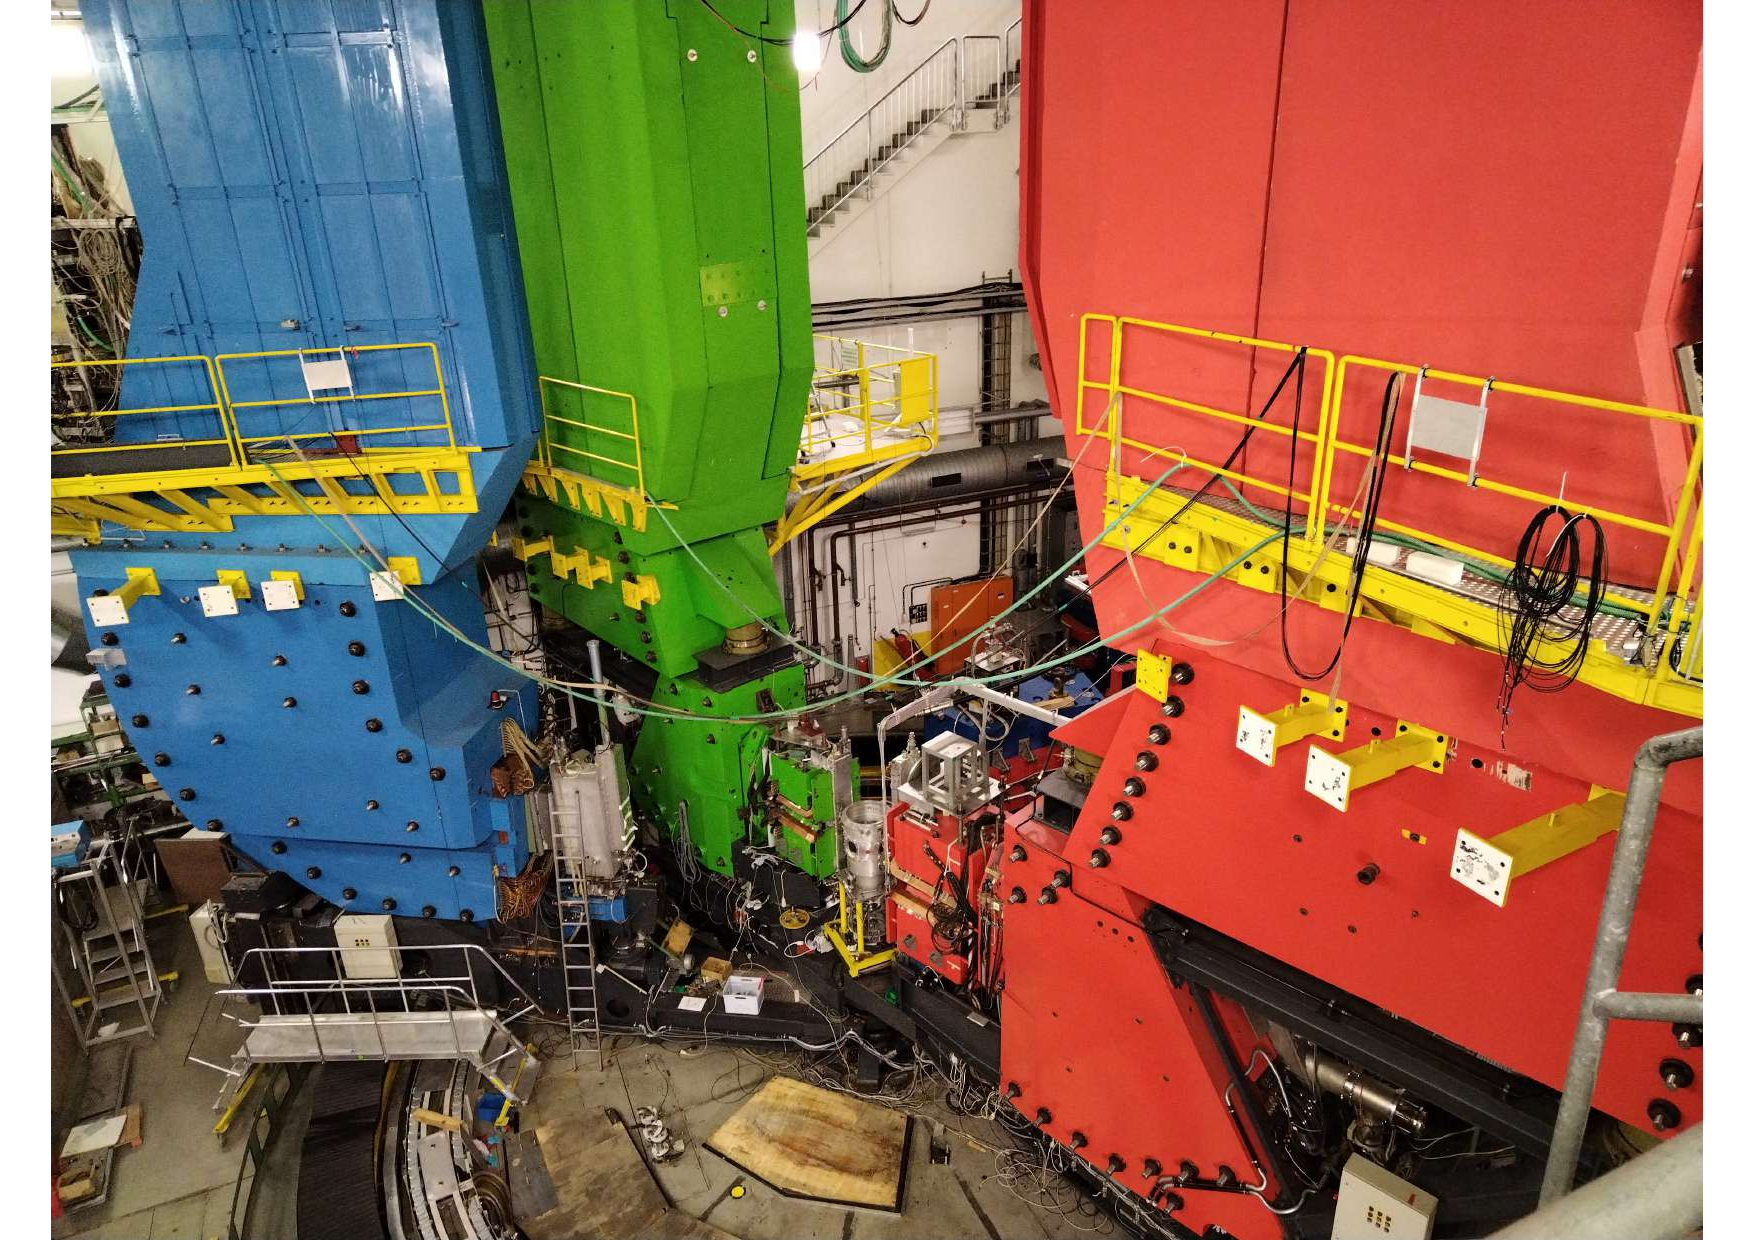
\includegraphics[width = 1\textwidth]{figures/twoSpektrometer.pdf}
\end{center}
\end{column}
\begin{column}{.5\textwidth}
\centering
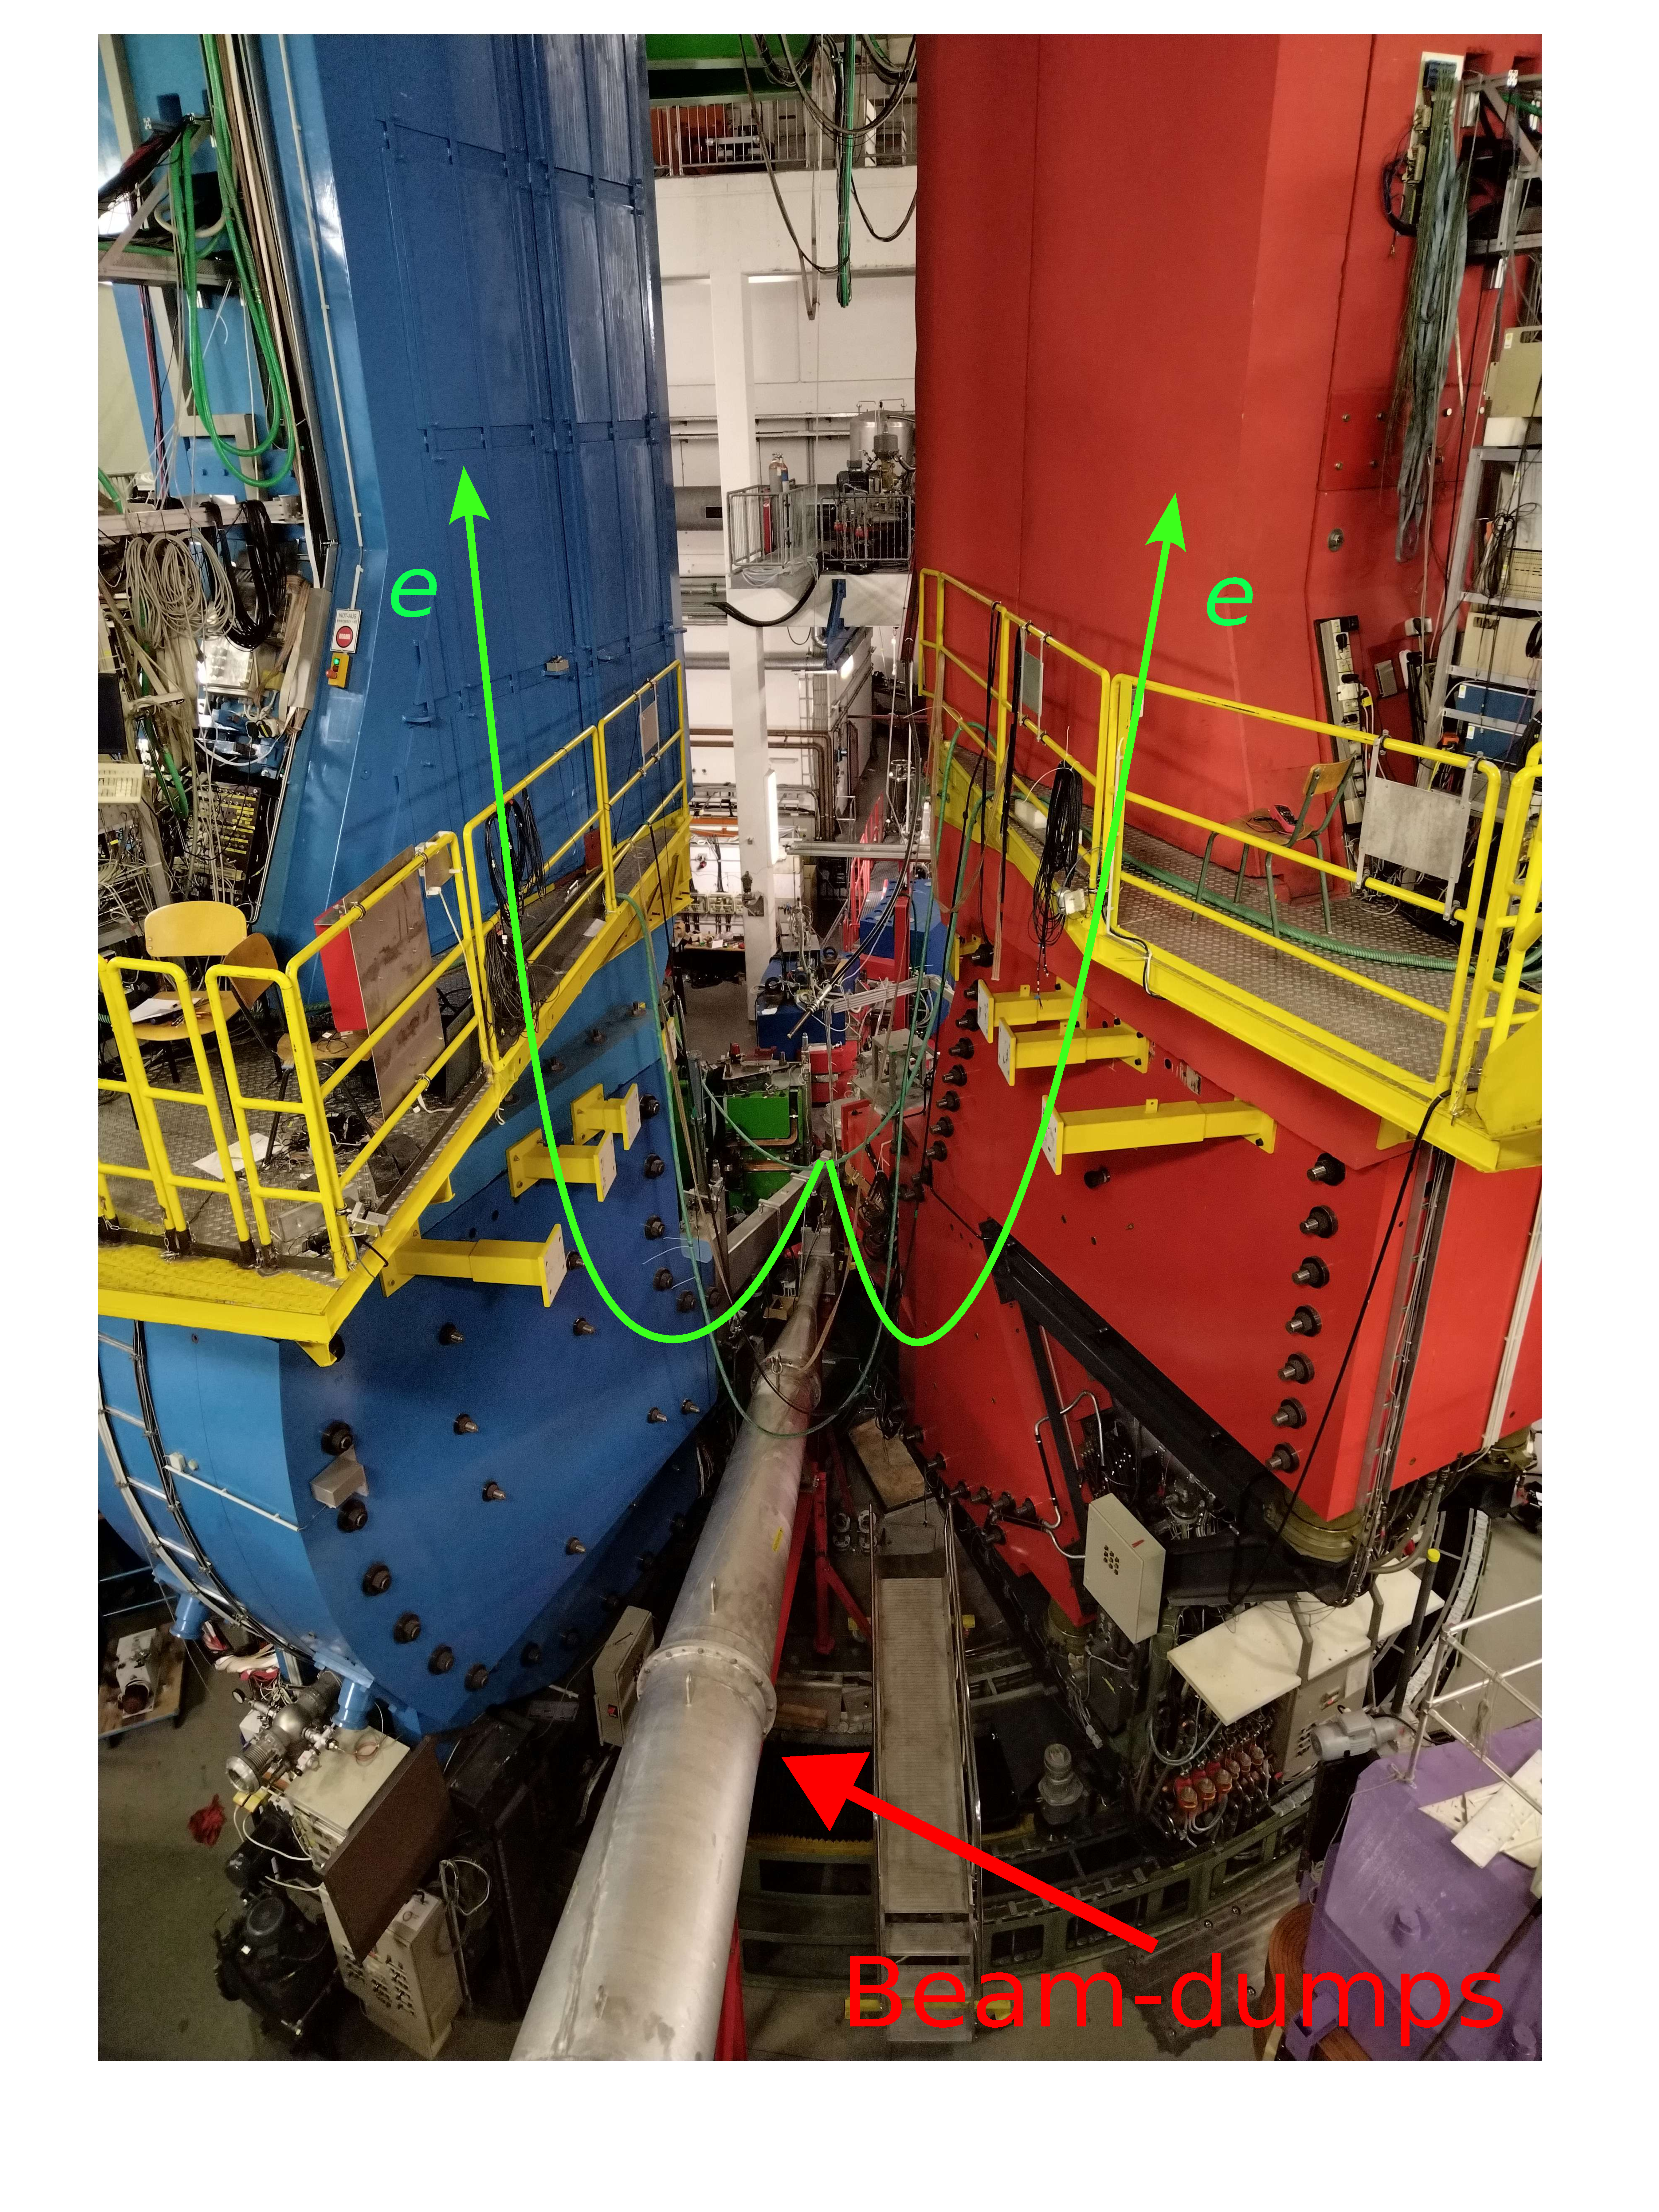
\includegraphics[width = 0.95\textwidth]{figures/A1_Dietro.pdf}
\end{column}
\end{columns}

\end{frame}

% 13 SCHEMA DETECTORS

\begin{frame}{Cherenkov Detectors}

\begin{figure}[!hbtp]
\centering
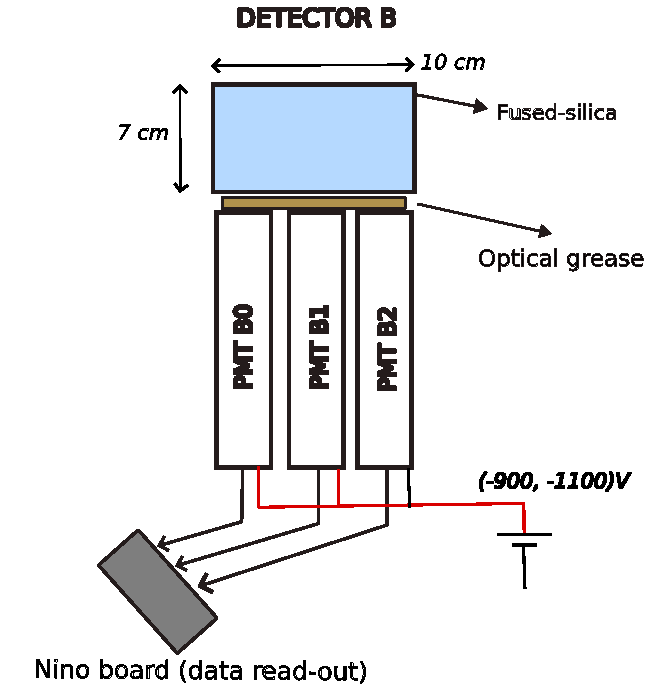
\includegraphics[width = 0.4\textwidth ]{figures/DetectorB.pdf}
\hspace{1cm}
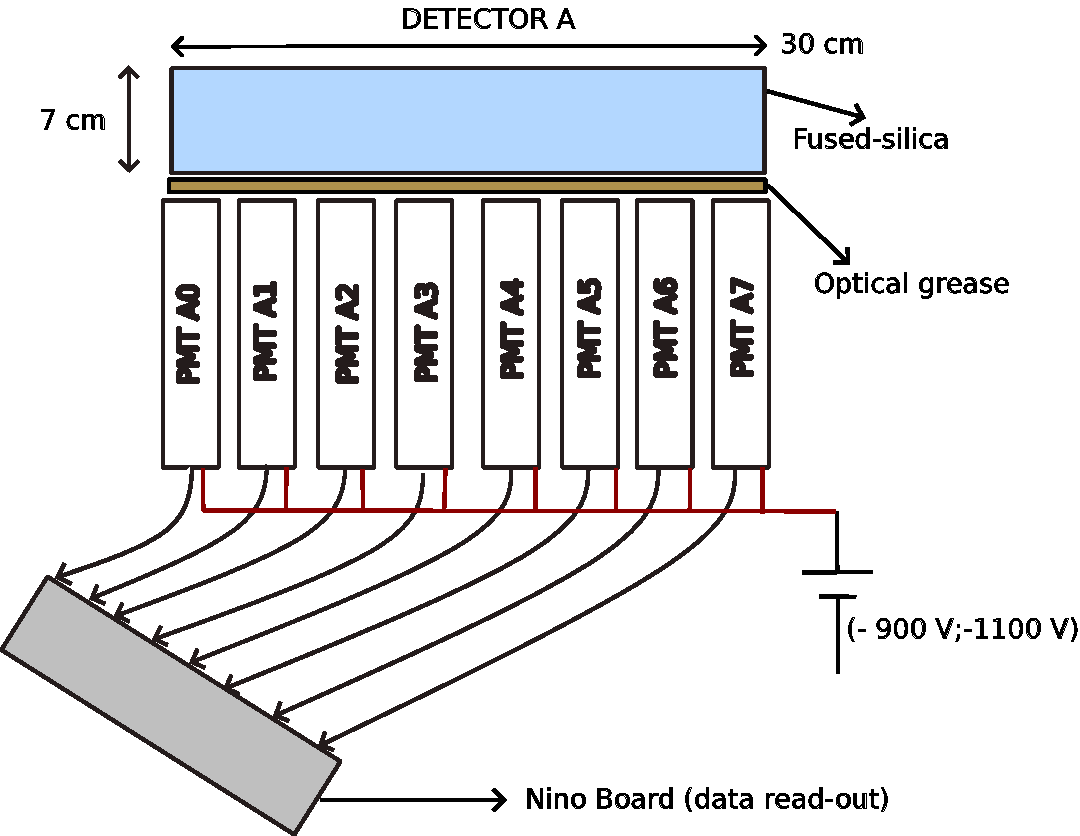
\includegraphics[width = 0.5\textwidth ]{figures/detectorA.pdf}
\caption{Scheme of detector B (on the left) and detector A (on the right).}
\end{figure}

\commento{The detectors are made by 9 and 3 pmts coupled to a fused-silica material, exploiting the Cherenkov light produced when a particle travel inside the material.

\begin{figure}[hbtp]
\centering
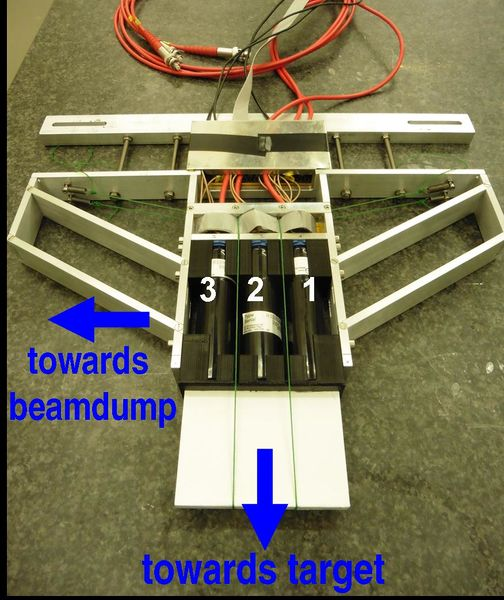
\includegraphics[width = 0.3\textwidth]{figures/504px-Blackfalcon.jpg}
\hspace{2cm}
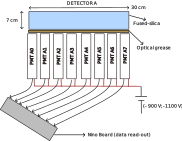
\includegraphics[width = 0.4\textwidth]{figures/DetectorA.jpg}
\caption{Detector B on the left, detector A on the right.}
\end{figure}}

\end{frame}

% 14 NINO BOARD
\begin{frame}[t]{NINO Asic Board}{Data Acquisition Electronics}
The NINO board is the DAQ system that counts the input signals coming from the Cherenkov detectors. 

\begin{itemize}
\item 32 input channels.
\item Attenuation circuit for each input channel.
\item Common current threshold for 4 adjacent channels.
\end{itemize}

\begin{center}
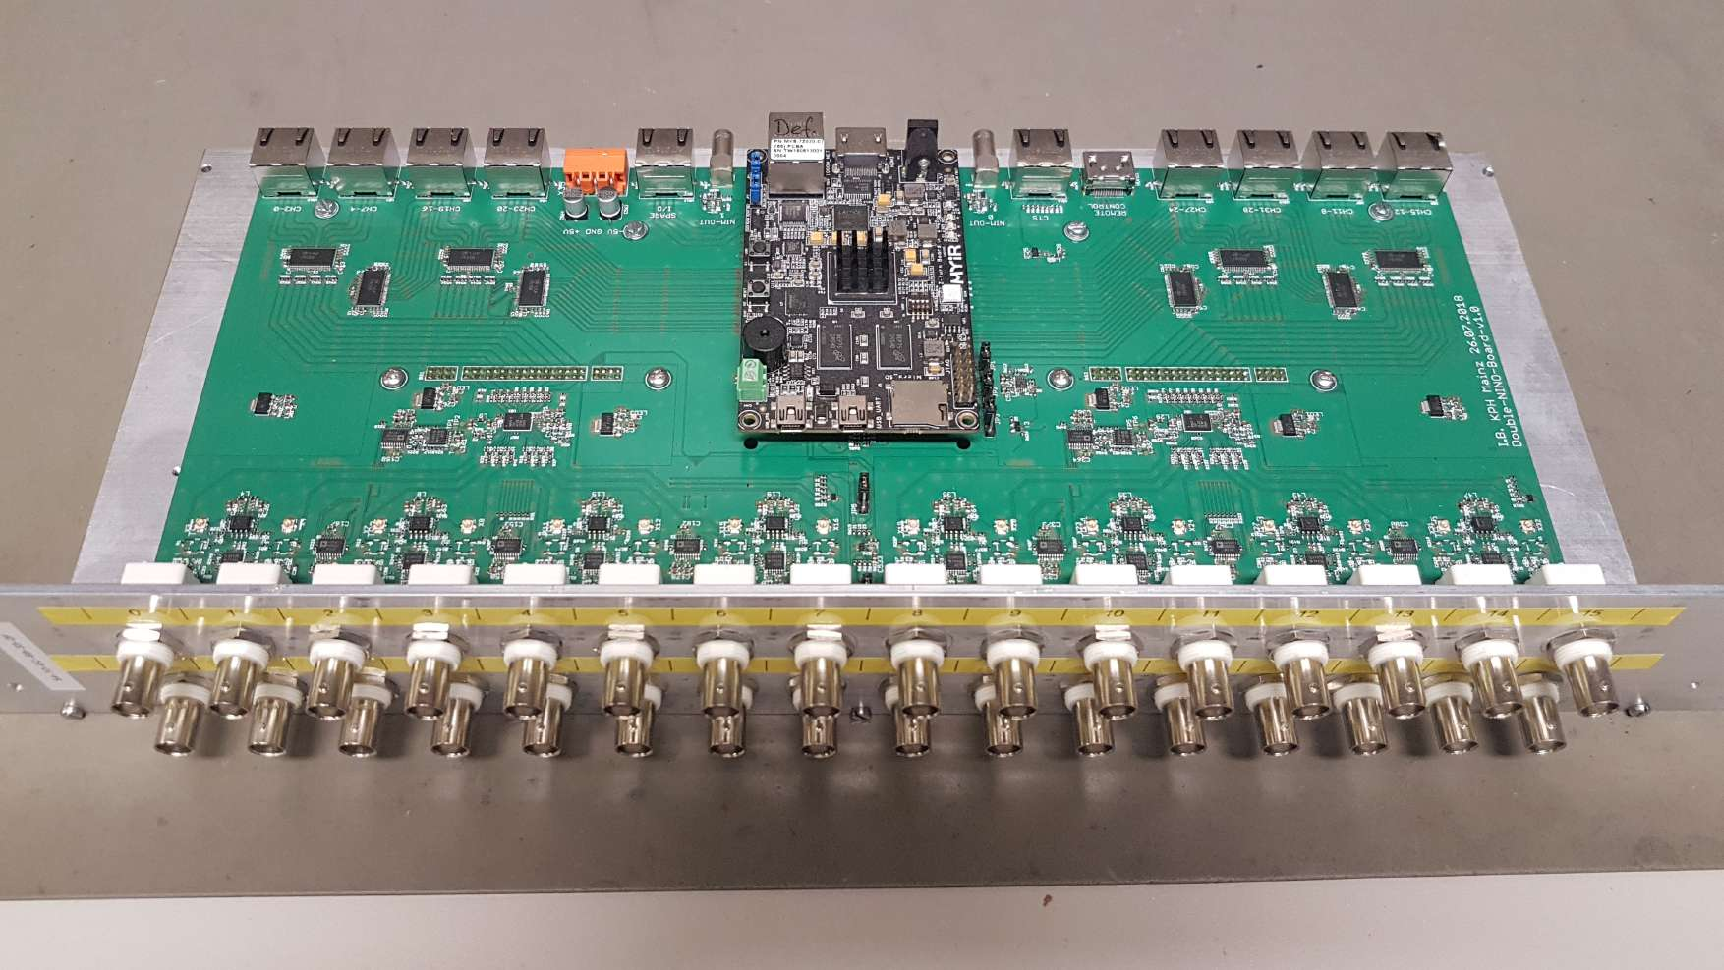
\includegraphics[width = 0.5\textwidth]{figures/NINO.pdf}
\end{center}
\end{frame}

\begin{frame}[t]{MAMI Beam Monitors}

At MAMI the beam parameters, as \textbf{X,Y} transverse positions, \textbf{Energy} and \textbf{Current} are measured by resonant cavities.

\begin{columns}[T]
\begin{column}{0.60\textwidth}
\begin{center}
\begin{figure}
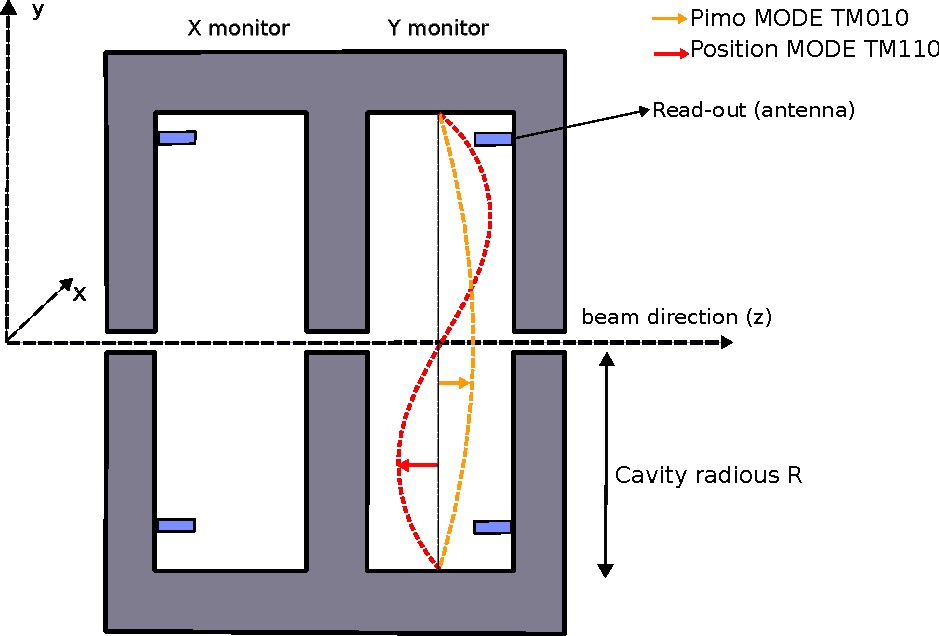
\includegraphics[width = 1\textwidth]{figures/Monitors.pdf}
\caption{Scheme of the resonant cavity in MAMI, with the different electromagnetic modes excited by the beam passage.}
\end{figure}
\end{center}
\end{column}
\begin{column}{0.40\textwidth}
The beam parameters are measured to take care of possible false asymmetries that arises from the variations of the beam parameters.
\end{column}
\end{columns}
\end{frame}

% 17 SCHEMA GENERALE DELL'ESPERIMENTO
\begin{frame}{General Scheme of the Experiment}

\begin{figure}[hbtp]
\centering
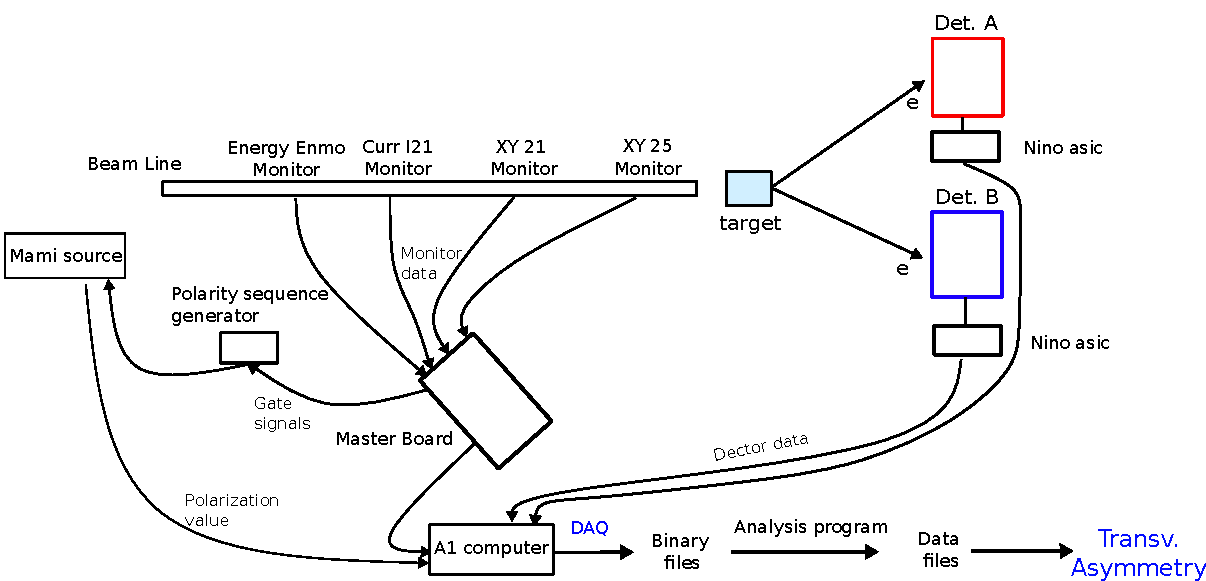
\includegraphics[width = 1\textwidth]{figures/Electronic_scheme.pdf}
\caption{Scheme of the experiment.}
\end{figure}
\end{frame}

% 18 1 DETECTOR TEST
\commento{
\begin{frame}{Detector Tests}

\end{frame}}

\begin{frame}[noframenumbering]{Data Analysis}
\begin{center}
\color{red}{\Large \bf{BEAM TIME AND CALIBRATIONS}}
\end{center}
\end{frame}

% 10 BEAM TIME, OBIETTIVI DELL'ESPERIMENTO
\begin{frame}{Beam-time 29/11/2022 - 5/12/2022}
\framesubtitle{Beam Normal Single Spin Asymmetry at MAMI}
During the last beam-time, several measurements were performed at Mainz Mikrotron MAMI. The last data acquisition campaign had the following goals:

\begin{itemize}
\item Test the new \textbf{data acquisition system}, developed for the new setup with a low rate signals ($\simeq \SI{1}{\mega \hertz} $). 
\item Measure the \textbf{transverse asymmetry} $A_{n}$ of $^{12}C$.
\item Measure the expected \textbf{rates} on $^{208}Pb$ target, in anticipation of the future measurement of $A_{n}$ for lead. 
\item Long term goal: acquire more knowledge on the \textbf{systematic effects} that the transverse asymmetry has on the measurement of the Parity-violating asymmetry.
\end{itemize}

Variation of the beam parameters can influence the measurements, inducing false asymmetries. These effects are corrected during the analysis. 
\end{frame}



% 16 Problema delle false asimmetrie
\commento{
\begin{frame}[t]{False Asymmetries}

Variation of the beam parameters can influence the measurements, inducing false asymmetries. The important parameters are:

\begin{itemize}
\item \textbf{X,Y} positions of the beam spot on the target.
\item beam current \textbf{I}.
\item beam energy \textbf{E}.
\item incident angles of the beam {$\bm{\theta_{x}},\bm{\theta_{y}}$}
\end{itemize}

Considering that the expected asymmetry is expected to be $\simeq 20 \, ppm$, small fluctuation of the beam correlated to the polarization can produce false asymmetries. The effects can be summarized by the model:
\begin{equation}
Asym = A_{physical} \cdot P + \delta_{I} + A_{x} \delta x + A_{y} \delta y + A_{\theta_{x}} \delta \theta_{x} + A_{\theta_{y}} \delta \theta_{y}+ A_{E} \delta E 
\end{equation}
\end{frame}}

% 18 CALIBRATION OF THE BEAM PARAMETERS
\begin{frame}{Calibration of the PMTs}{working point of the PMTS}

\begin{figure}
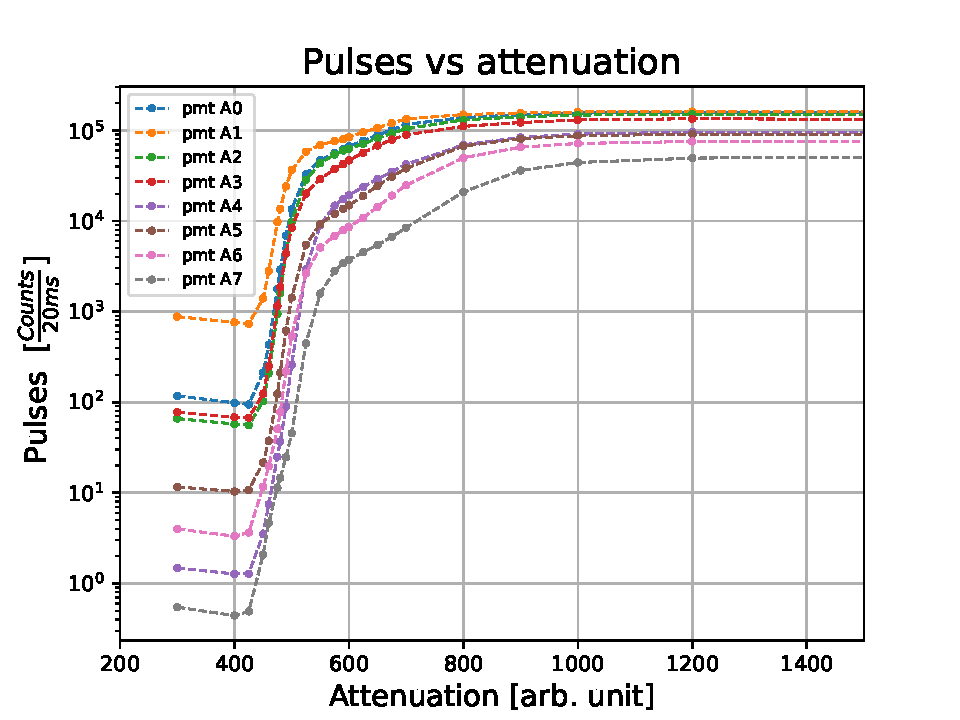
\includegraphics[width = 0.4\textwidth]{figures/AttenuationScanA.pdf}
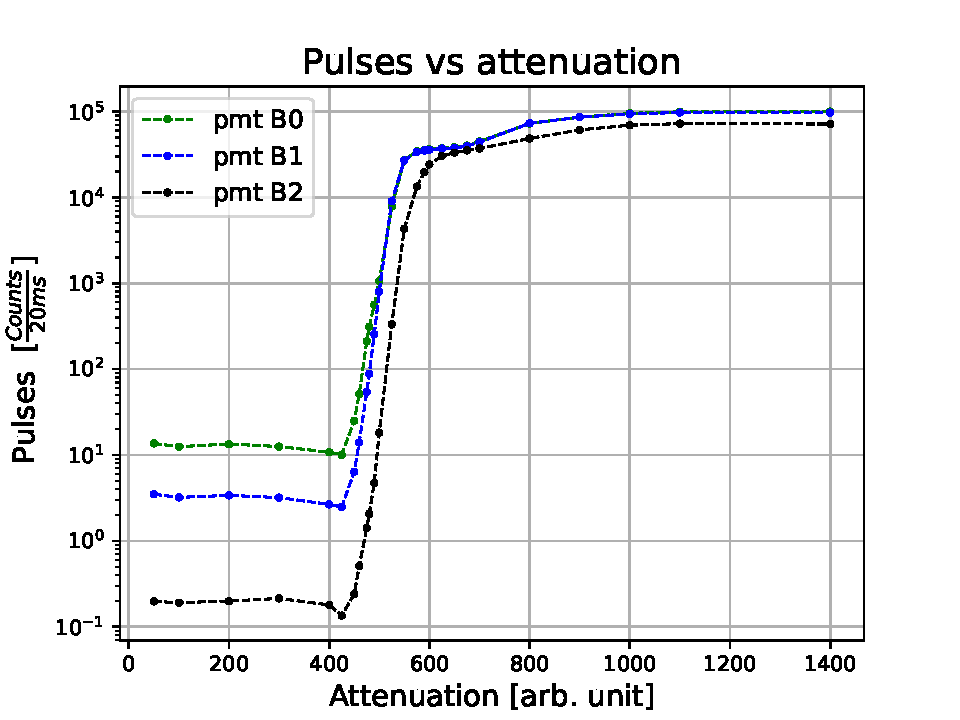
\includegraphics[width = 0.4\textwidth]{figures/AttenuationScanB.pdf}
\caption{\footnotesize Counts versus attenuation value for PMTs of detector A (left plot) and B (right plot).}
\end{figure}

\begin{figure}
\centering
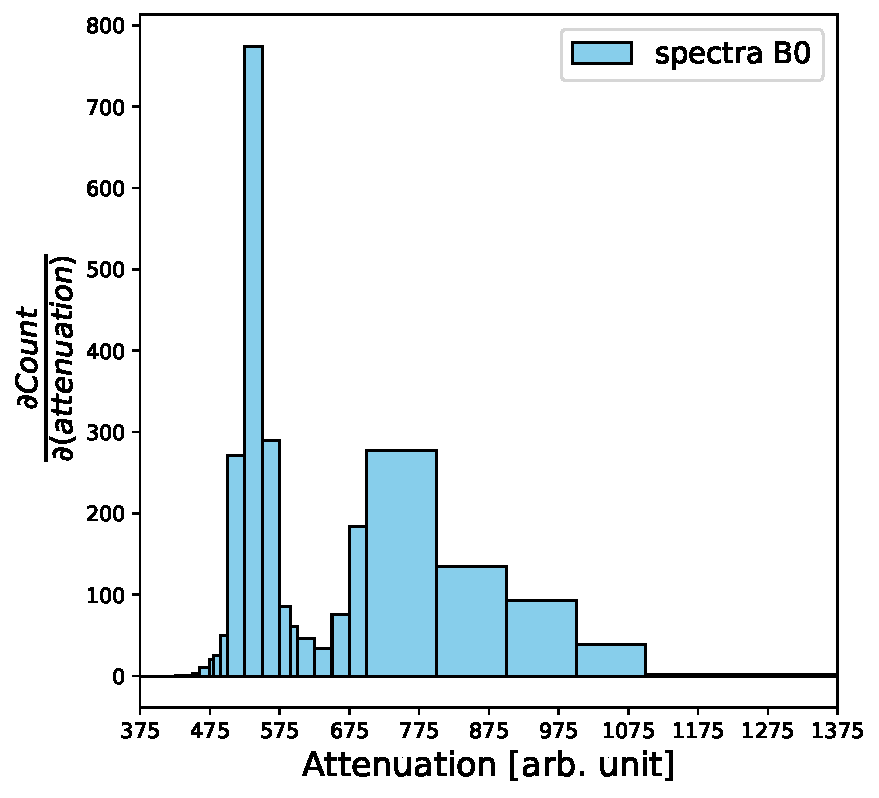
\includegraphics[width = 0.25\textwidth]{figures/spettro/B0.pdf}
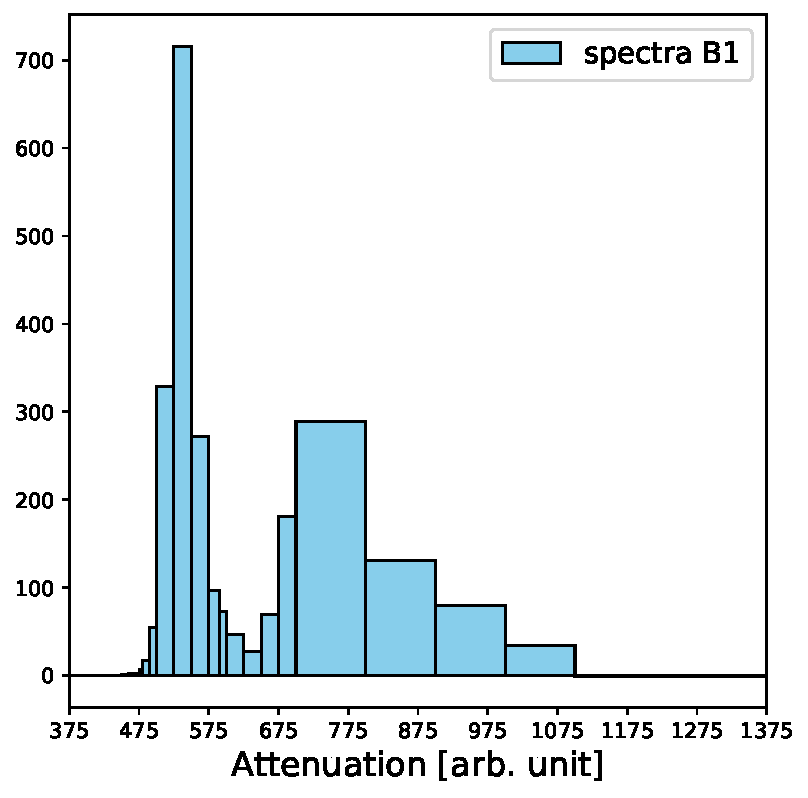
\includegraphics[width = 0.23\textwidth]{figures/spettro/B1.pdf}
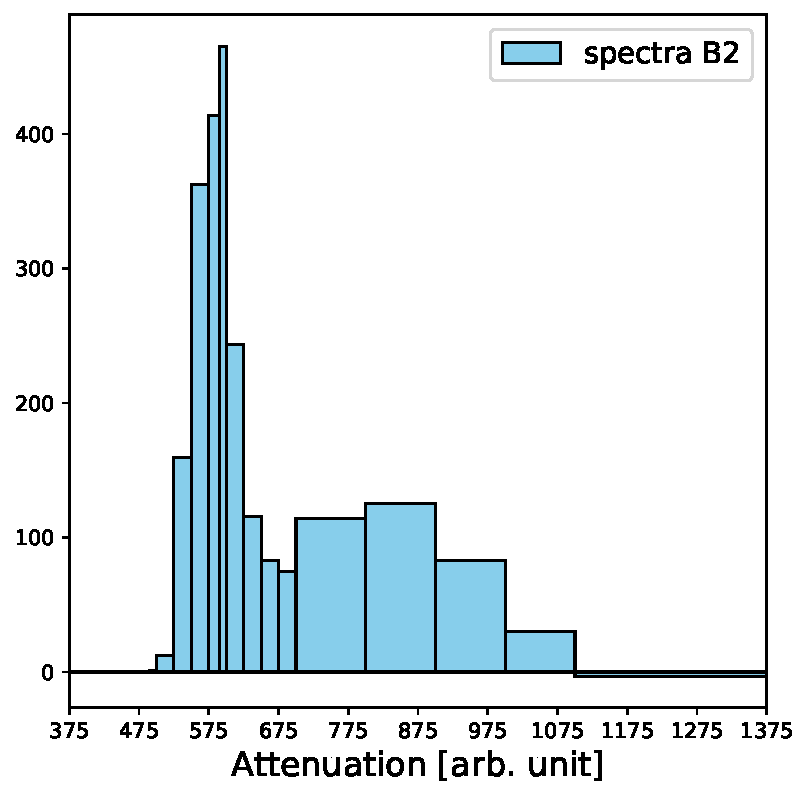
\includegraphics[width = 0.23\textwidth]{figures/spettro/B2.pdf}
\end{figure}
\end{frame}

\begin{frame}{Calibration of the Beam Monitors}{Beam Position (X,Y) on the target}
\begin{figure}
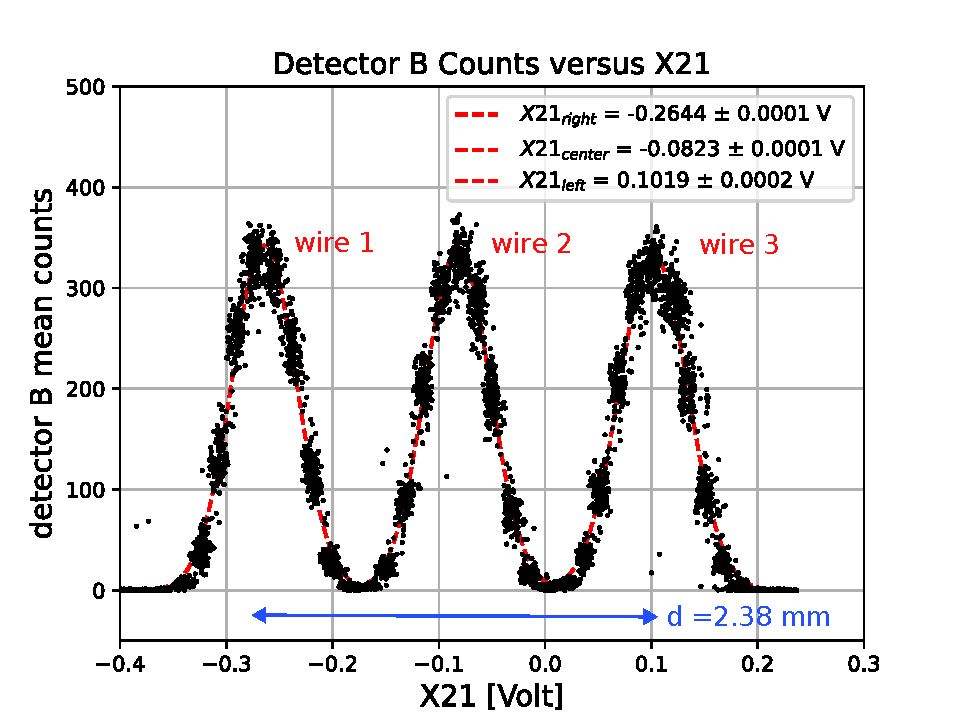
\includegraphics[width = 0.70\textwidth]{figures/HorizontalCalibration.pdf}
\caption{\footnotesize Calibration of the X21 monitor.}
\end{figure}
\end{frame}

\begin{frame}{Calibration of the Beam Monitors}{Beam Position (X,Y) on the target}

\begin{figure}[hbtp]
\centering
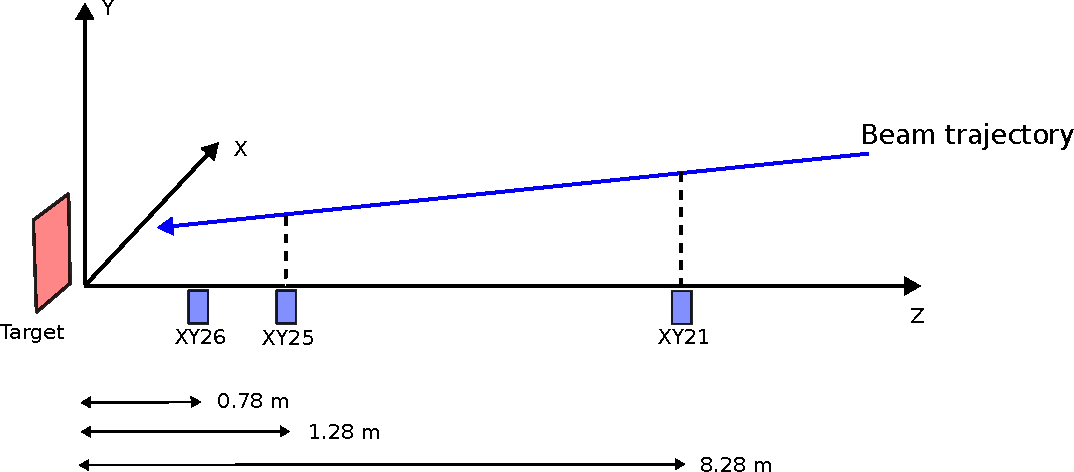
\includegraphics[width = 0.9\textwidth]{figures/scheme.pdf}
\end{figure}

The beam is assumed following a straight path given by $x,y = m\cdot z + q_{x,y}$, the $(X,Y)$ coordinates are given by $q_{x,y}$

\end{frame}

\begin{frame}{Beam Energy and Beam Current}

The conversion parameters from \SI{}{\volt} to \SI{}{\micro \ampere} and \SI{}{\kilo \electronvolt} are measured with a current and energy scan.

\begin{columns}
\begin{column}{0.5\textwidth}
\begin{figure}
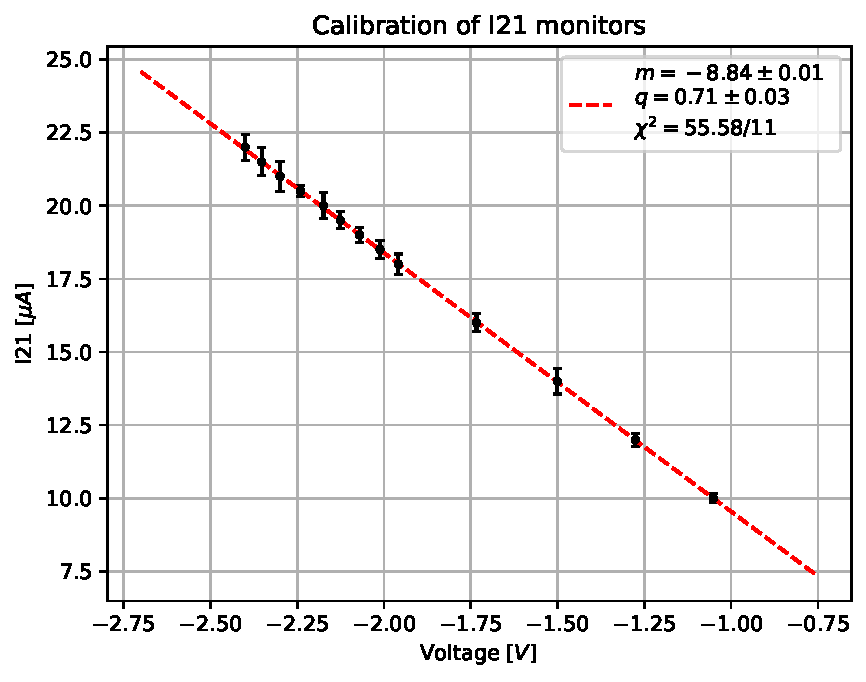
\includegraphics[width = 0.95\textwidth]{figures/I21.pdf}
\caption{ \footnotesize Current monitor I21. On the x axis the voltage signal of the PIMO monitor, on the y axis the nominal current of the beam.}
\end{figure}
\end{column}
\begin{column}{0.5\textwidth}
\begin{figure}
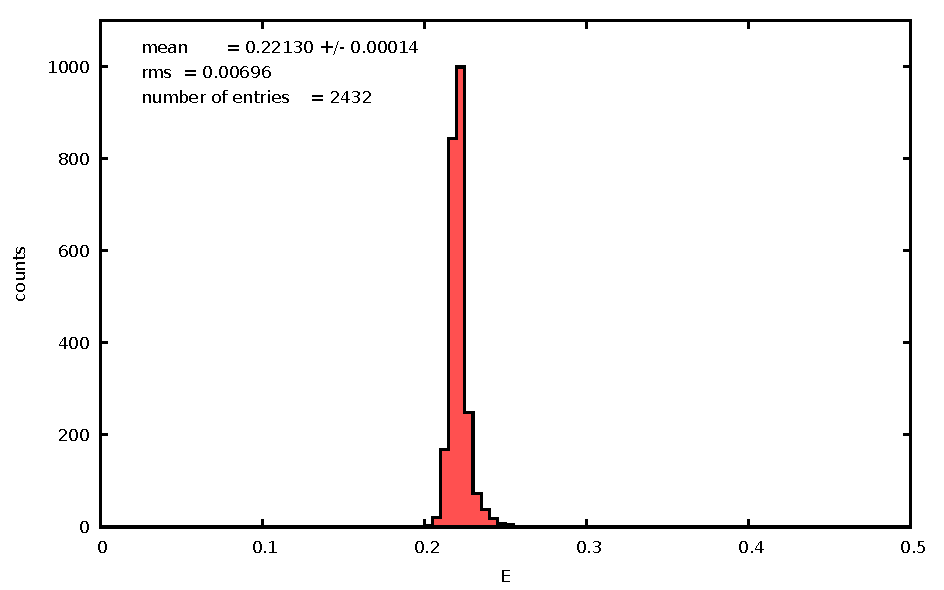
\includegraphics[width = 0.75\textwidth]{figures/ENMOvoltage15.pdf}
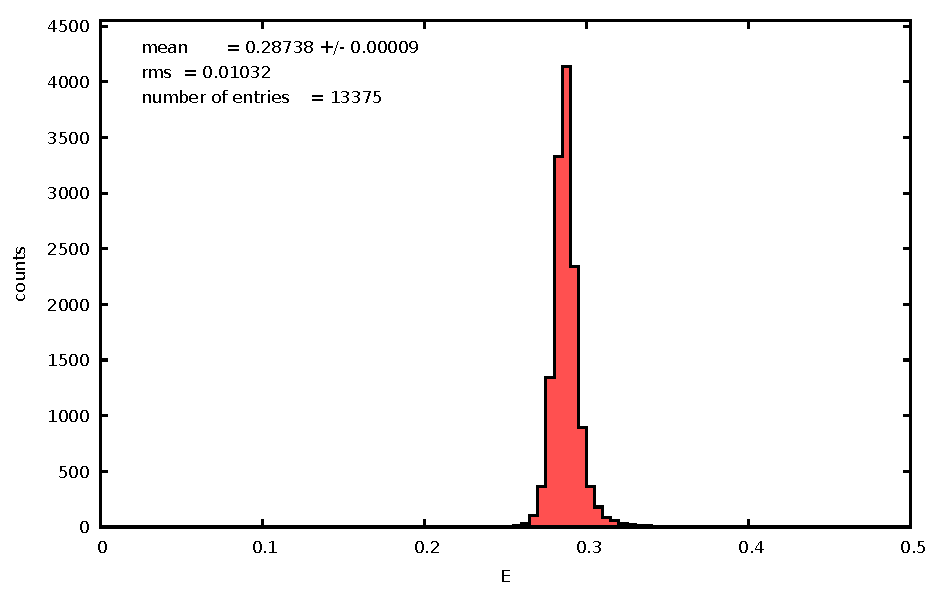
\includegraphics[width = 0.75\textwidth]{figures/ENMOvoltage20.pdf}
\caption{\footnotesize Calibration of the energy monitor. For the first histogram the current is \SI{15}{\micro \ampere}, \SI{20}{\micro \ampere} for the second one.}
\end{figure}
\end{column}
\end{columns}

\end{frame}

\begin{frame}{Auto-Calibration procedure}

Every 3 hours of beam, a special operation mode of MAMI is set. The current is raised in small steps, from $\SI{9}{\micro \ampere}$ to $\SI{11.125}{\micro \ampere}$. This is used to check the linearity of the PMTs through time, and to measure the PMT offset, that is subtracted later from the data.

\begin{columns}
\begin{column}{0.5\textwidth}
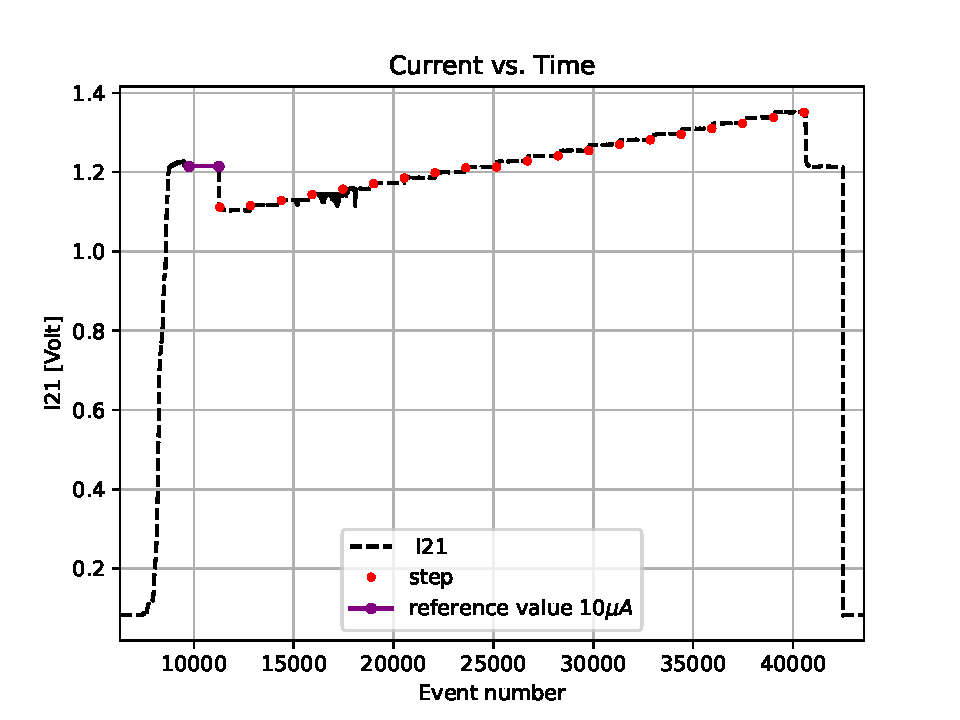
\includegraphics[width = \textwidth]{figures/Current.pdf}
\end{column}
\begin{column}{0.5\textwidth}
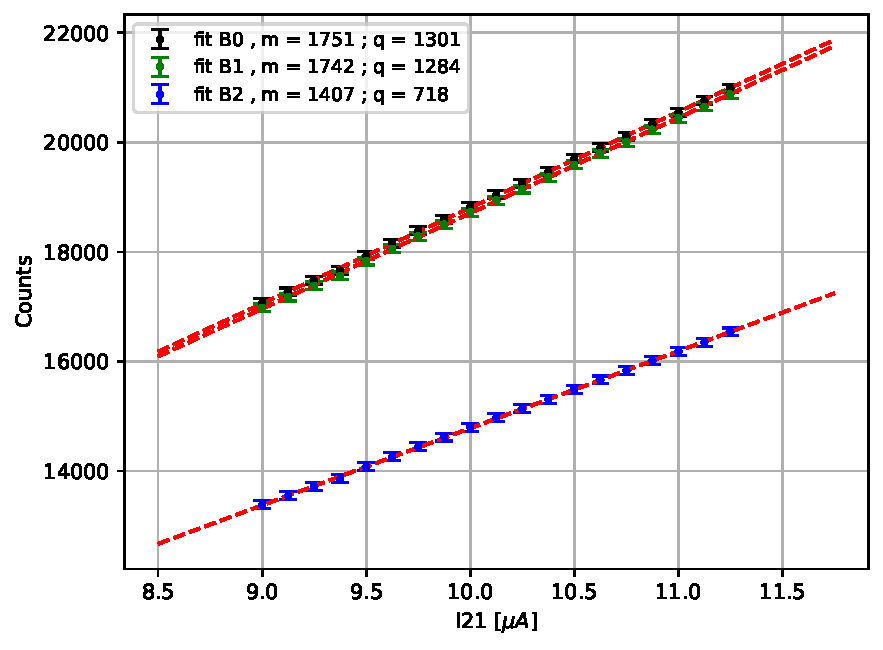
\includegraphics[width = 0.9\textwidth]{figures/fitB.pdf}
\end{column}
\end{columns}

\end{frame}

% DATA ANALYSIS
\begin{frame}[noframenumbering]{Data Analysis}
\begin{center}
\color{red}{\Large \bf{DATA ANALYSIS}}
\end{center}
\end{frame}

% 15 Struttura dell'evento
\begin{frame}{Structure of the event}

\begin{equation}
A_{mes.} = \dfrac{(N_{1} + N_{4}) - (N_{2} + N_{3})}{(N_{1} + N_{4}) + (N_{2} + N_{3})}
\end{equation}

The Data are divided in a series of events (\SI{80}{\milli \second}), that correspond to 4 sequential sub-event. For each sub-event there is a precise polarization of the Beam. During the \SI{20}{\milli \second} of the sub-event, all the electrons are counted. 

\begin{figure}[hbtp]
\centering
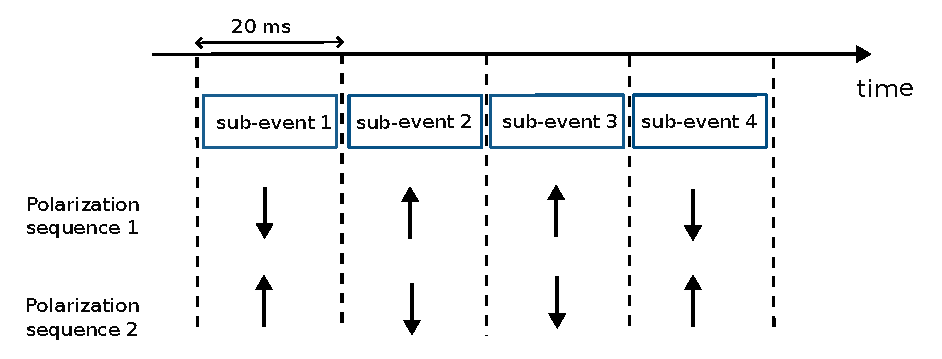
\includegraphics[width = 0.85\textwidth]{figures/EventStructure.pdf}
\caption{Event sequence}
\end{figure}
\end{frame}

\begin{frame}[t]{Analysis on Carbon Target}

Each event corresponds to a single measurement of the asymmetry $A$. With this experiment, an amount of $1$ million events have been collected. The asymmetry data are normal distributed:

\begin{columns}
\begin{column}{0.5\textwidth}
\begin{figure}
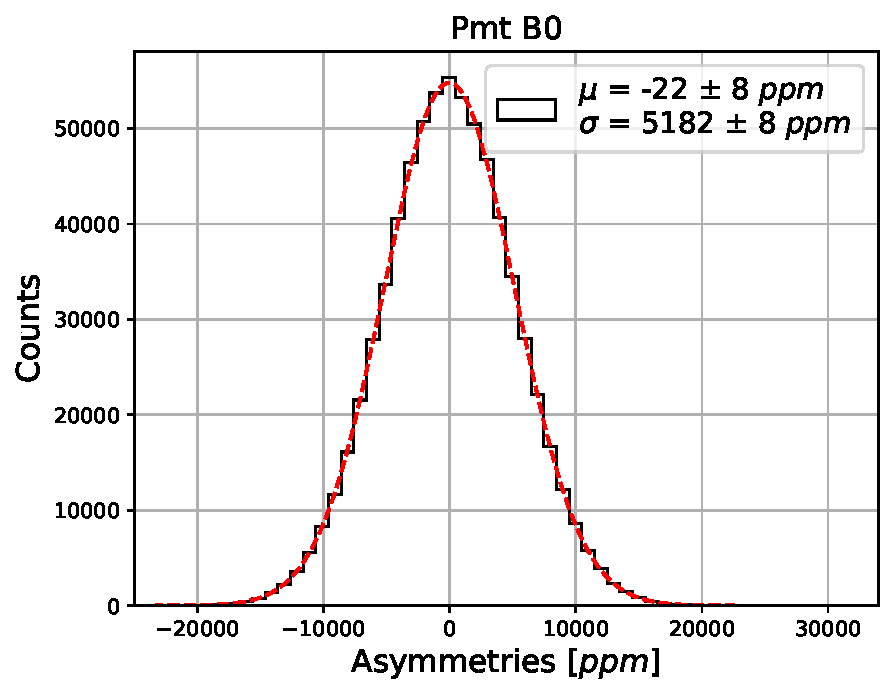
\includegraphics[width = \textwidth]{figures/B0.pdf}
\end{figure}
\end{column}
\begin{column}{0.5\textwidth}
\begin{gather*}
Var[A_{asym}] = Var[\dfrac{N_{\uparrow} - N_{\downarrow}}{ N_{\uparrow} + N_{\downarrow}}] \simeq \dfrac{Var[N_{\uparrow} - N_{\downarrow}]}{(N_{\uparrow} + N_{\downarrow})^{2}} \\
\frac{2Var[N]}{4N^{2}} = \frac{1}{2N} \qquad \sigma = \frac{1}{\sqrt{2N}}
\end{gather*}

Where it is supposed that the PMTs counts are normal distributed, with $\mu$ equal to $\sigma^{2}$. The rms associated to the sample mean decreases as the $\sqrt{N_{measure}}$. With the statistical error is:

\begin{equation}
\sigma = \dfrac{1}{\sqrt{2 N \cdot N_{measure}}} 
\end{equation}
\end{column}
\end{columns}

Considering $5\cdot 10^{5}$ events and $\mu = 20000$ counts per PMT (similar to what was measured for detector B) 

\begin{itemize}
\centering
\item $\sigma = 8 \, ppm$.
\end{itemize}
\end{frame}

% 20 Model for Fitting the Data
\begin{frame}[t]{Model For Fitting the Data}

Considering that $A$ for $^{12}C$ is expected to be $\simeq 20 \, ppm$, small fluctuations of the beam correlated to the polarization can produce false asymmetries. The important parameters are:

\begin{itemize}
\item \textbf{X,Y} positions of the beam spot on the target.
\item beam current \textbf{I}.
\item beam energy \textbf{E}.
\item incident angles of the beam {$\bm{\theta_{x}},\bm{\theta_{y}}$}
\end{itemize}

The final model assumes a \textbf{linear dependence} on the beam parameters:

\begin{equation}
A_{tot} = A_{physical} \cdot P + \delta_{I} + A_{x} \delta x + A_{y} \delta y + A_{\theta_{x}} \delta \theta_{x} + A_{\theta_{y}} \delta \theta_{y}+ A_{E} \delta E 
\end{equation}

Each $\delta q$ is computed as the mean difference between up and down polarized sub-events:

\begin{equation}
\delta q = \dfrac{q_{\uparrow,0} + q_{\uparrow,1}}{2} - \dfrac{q_{\downarrow,0} + q_{\downarrow,1}}{2}
\end{equation}

The current asymmetry is defined differently. Because the scattering rate is proportional to the beam current, the model contains the current asymmetry directly:

\begin{equation}
\delta I = \dfrac{I_{\uparrow} - I_{\downarrow}}{I_{\uparrow} + I_{\downarrow}}
\end{equation}

\end{frame}

% 23 FIT TO DATA, CORRELATION
\begin{frame}{Beam Parameters Correlation}

\begin{figure}
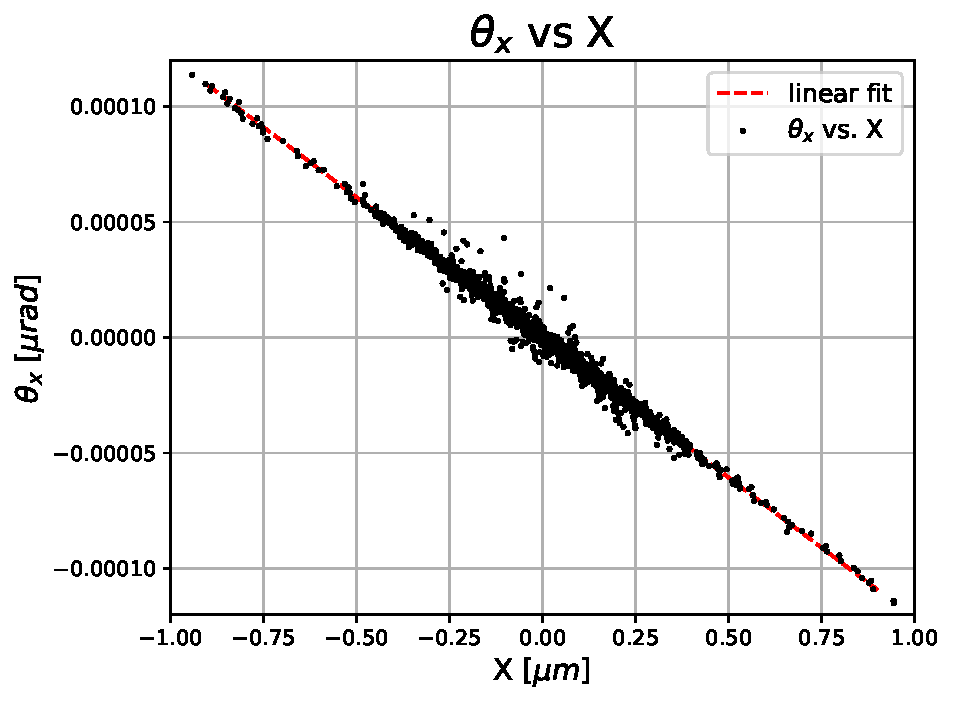
\includegraphics[width = 0.4\textwidth]{figures/X_Xp.pdf}
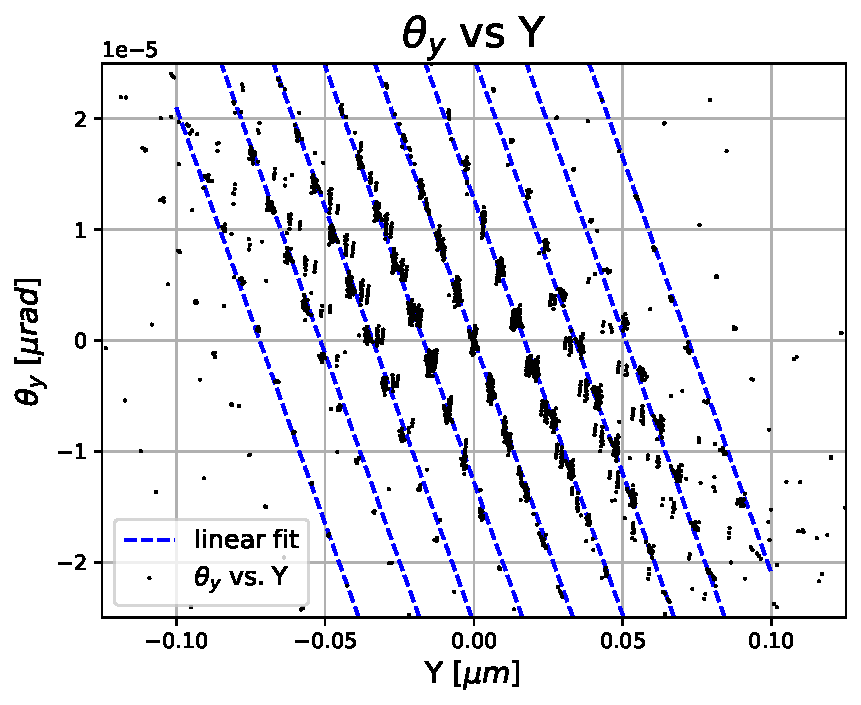
\includegraphics[width = 0.37\textwidth]{figures/Y_Yp.pdf} \\
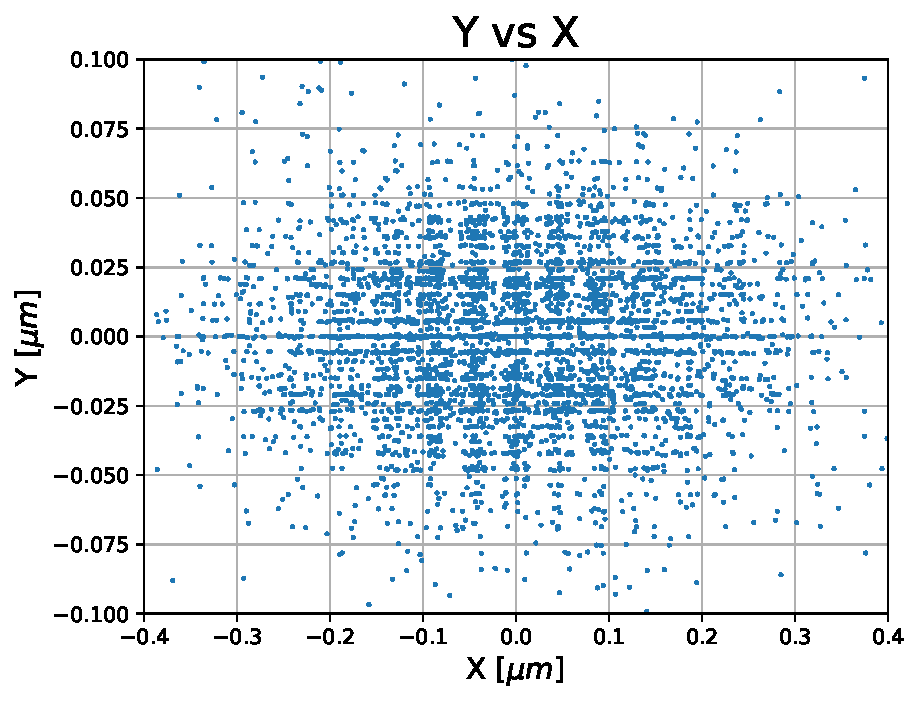
\includegraphics[width = 0.4\textwidth]{figures/Y_X.pdf}
\end{figure}
\end{frame}

% 21 Data Selection
\begin{frame}{Data Selection}
Before proceeding in the analysis, an accurate data selection was performed, to remove the outliers, as well as data affected by anomalous variation of the beam current or polarization loss.

\begin{columns}
\begin{column}{0.5\textwidth}
\begin{figure}
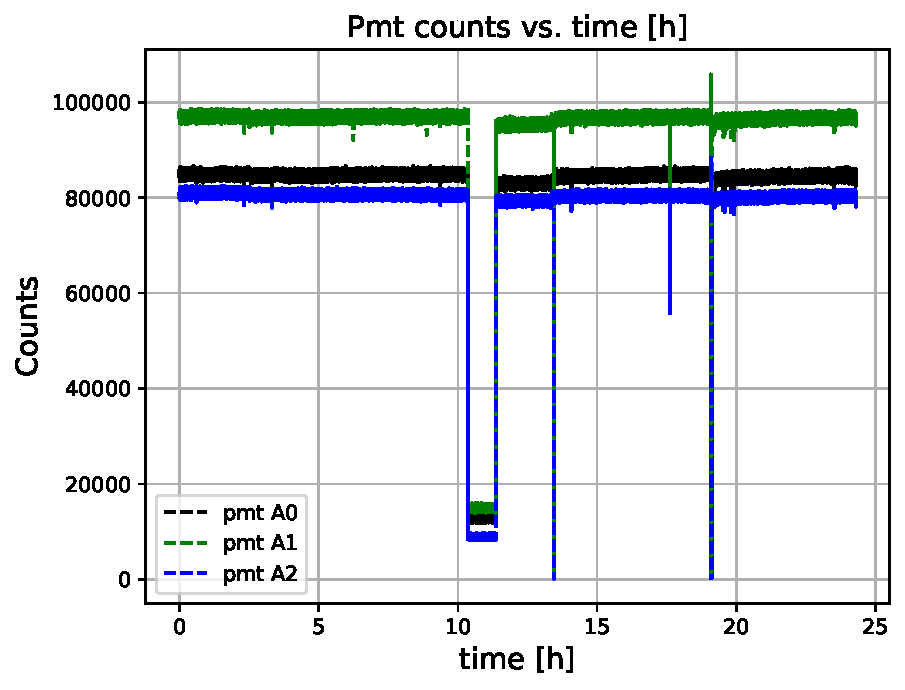
\includegraphics[width = 1\textwidth]{figures/BeamExample.pdf}
\caption{PMT counts of detector B versus time.}
\end{figure}
\end{column}
\begin{column}{0.5\textwidth}
\begin{figure}
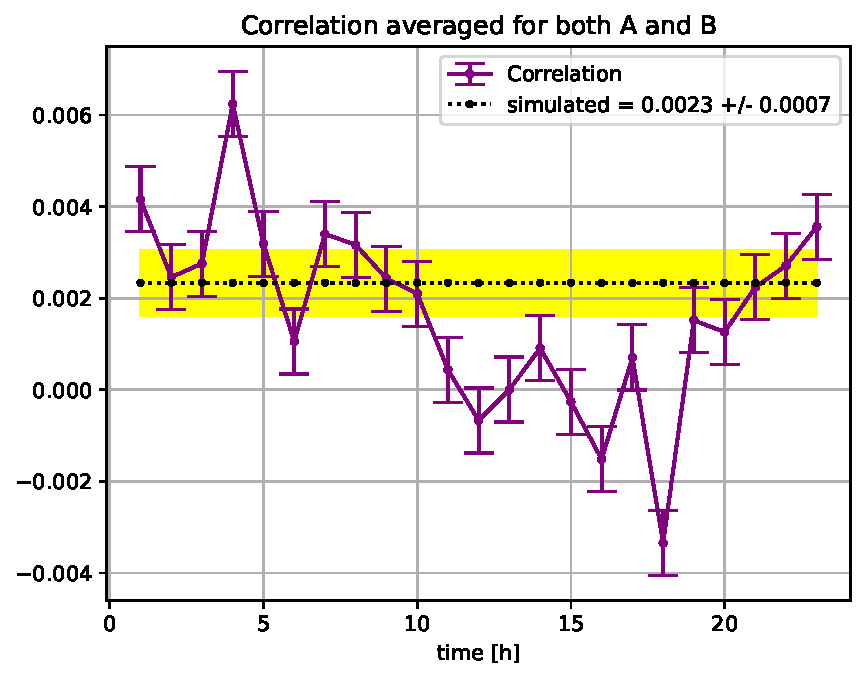
\includegraphics[width = 1\textwidth]{figures/OverallCorr.pdf}
\caption{Correlation between the PMTs counts and the polarization. A loss of beam polarization can be identified at $t = 11 \, h$.}
\end{figure}
\end{column}
\end{columns}
\end{frame}

\begin{frame}{Results}
\begin{center}
Final asymmetry result for each PMTs:
\end{center}
\begin{center}
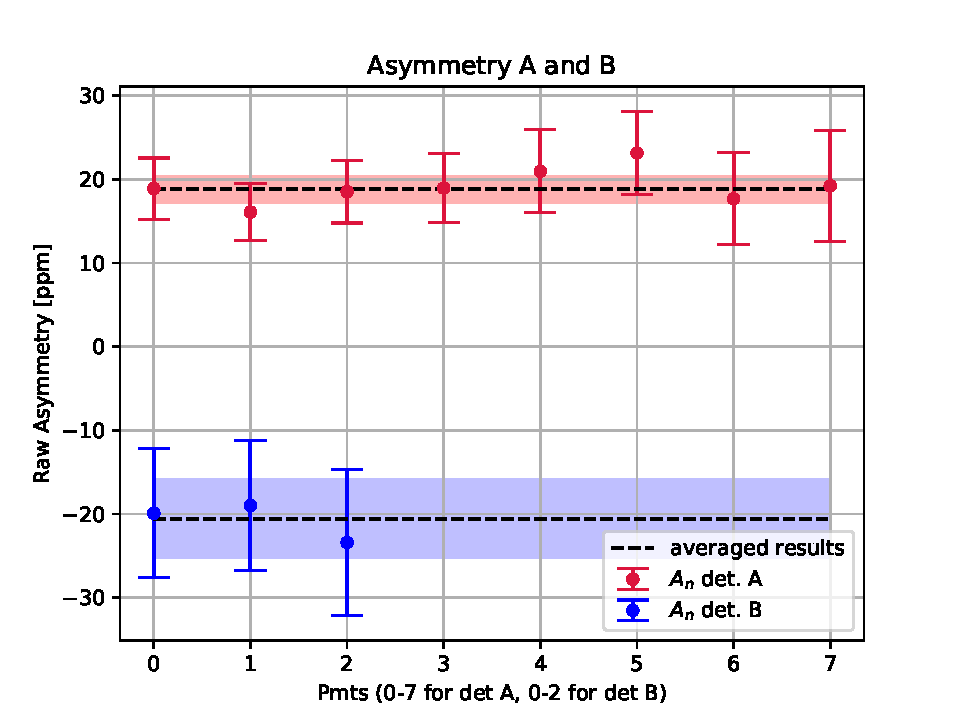
\includegraphics[width = 0.80\textwidth]{figures/FirstResult.pdf}
\end{center}

\end{frame}

\begin{frame}{Results}

The result of the analysis is obtained combining the measured asymmetries for PMTs. 

\begin{gather*}
\hat{A} =  \frac{\Sigma_{i} A_{i} \frac{1}{w_{i}}}{\frac{1}{w_{i}}} \qquad w_{i} = \frac{1}{\sigma^{2}_{i}}
\end{gather*}

the final values of the Beam Normal Single Spin asymmetries are:

\begin{equation}
A_{A} = 23.1 \pm 1.7 \, ppm  \qquad A_{B} = -21 \pm 5 \, ppm
\end{equation}

With a transfer momentum $Q = \SI{0.04}{\giga \electronvolt}$. Reversing the sign of the asymmetry for Det. B we notice that the two measurement are consistent within $1 \, \sigma$. The values measured in this thesis work are in agreement with precedent measurement performed at MAMI, with the old electronic setup:

\begin{equation}
A_{A} = 23.9 \pm 1(stat) \pm 0.7 (syst) \, ppm  \qquad A_{B} = -21.9 \pm 1.5(stat) \pm 1.6(syst) \, ppm
\end{equation}


\end{frame}

\begin{frame}[noframenumbering]{Ringraziamenti}
\begin{center}
\color{red}{\Large \bf{GRAZIE A TUTTI PER L'ATTENZIONE}}
\end{center}
\end{frame}

\begin{frame}[noframenumbering]
\begin{center}
\color{red}{\Large \bf{ADDITIONAL MATERIAL}}
\end{center}
\end{frame}

\begin{frame}[noframenumbering]{Rates on Lead}

The rates on lead target (\SI{1}{\milli \meter} thick) have been measured. The transverse asymmetry on lead will be the next step of MREX experiment. This measurement is mandatory to constrain the systematic error of PV experiment.

\begin{figure}[hbtp]
\centering
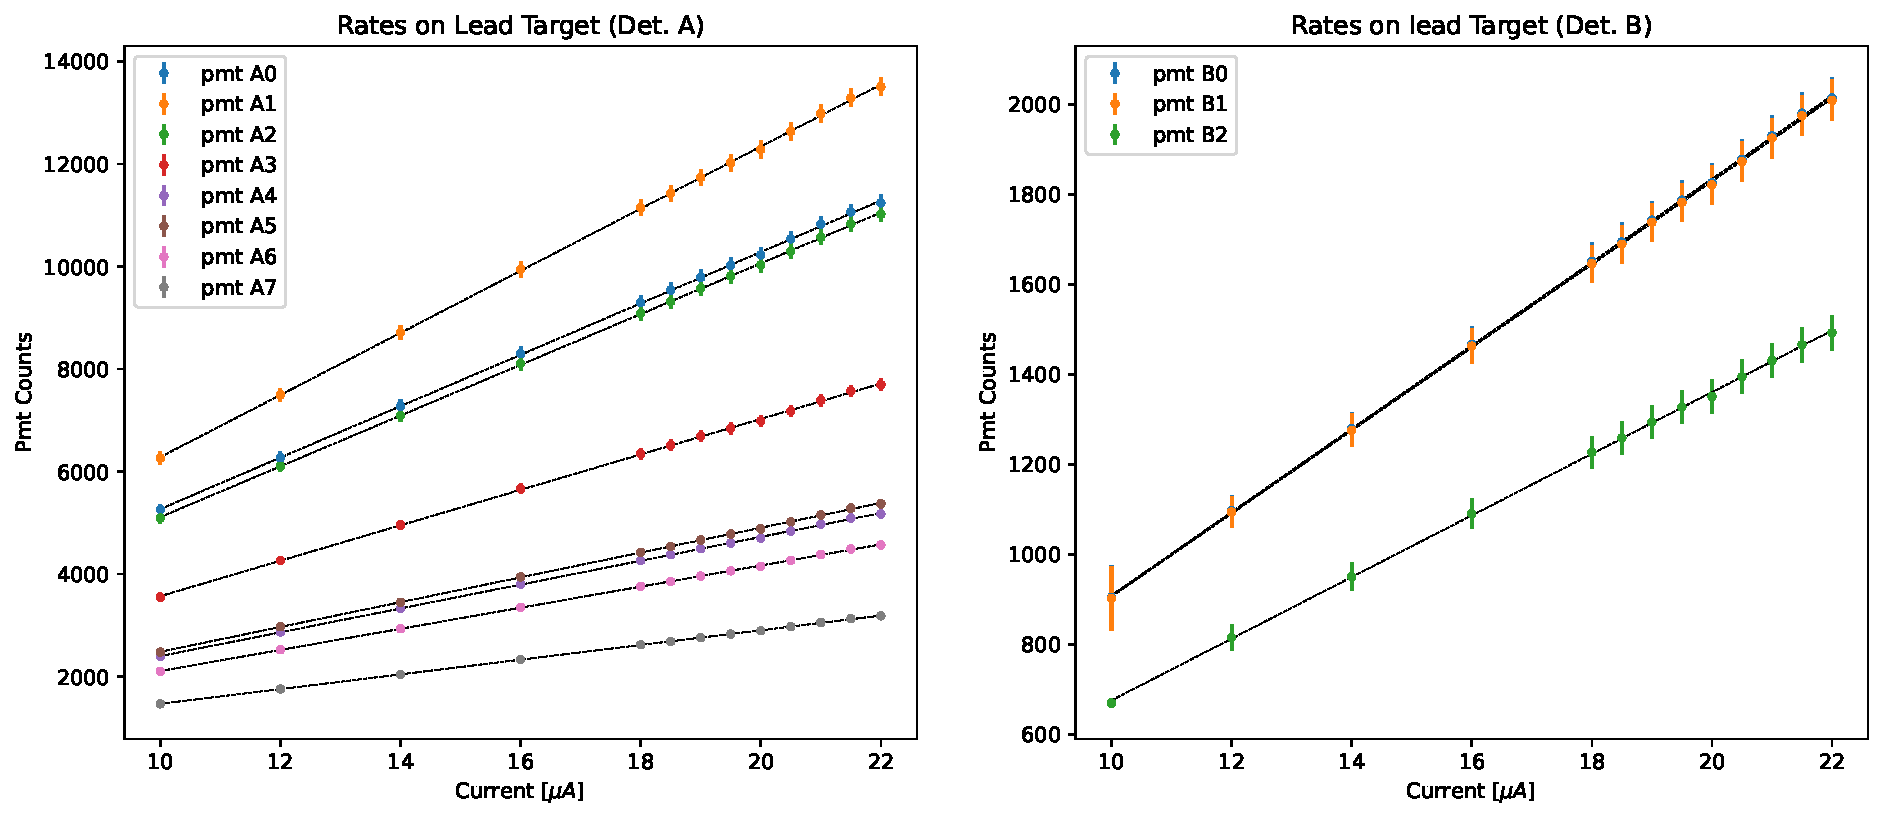
\includegraphics[width = \textwidth]{figures/LeadRates.pdf}
\end{figure}

Since the rates are lower for lead compared to carbon, the statistics needed to measure $A_{n}$ for $^{208}Pb$ is 23 times the statistic accumulated for carbon.
\end{frame}

\begin{frame}[noframenumbering]

Here a plot about the trend of the asymmetry as the data increases. The band is the error computed as showed in the previous slide, centered around the values of $+20ppm$ for detector A and $-20ppm$ for detector B.

\begin{figure}[hbtp]
\centering
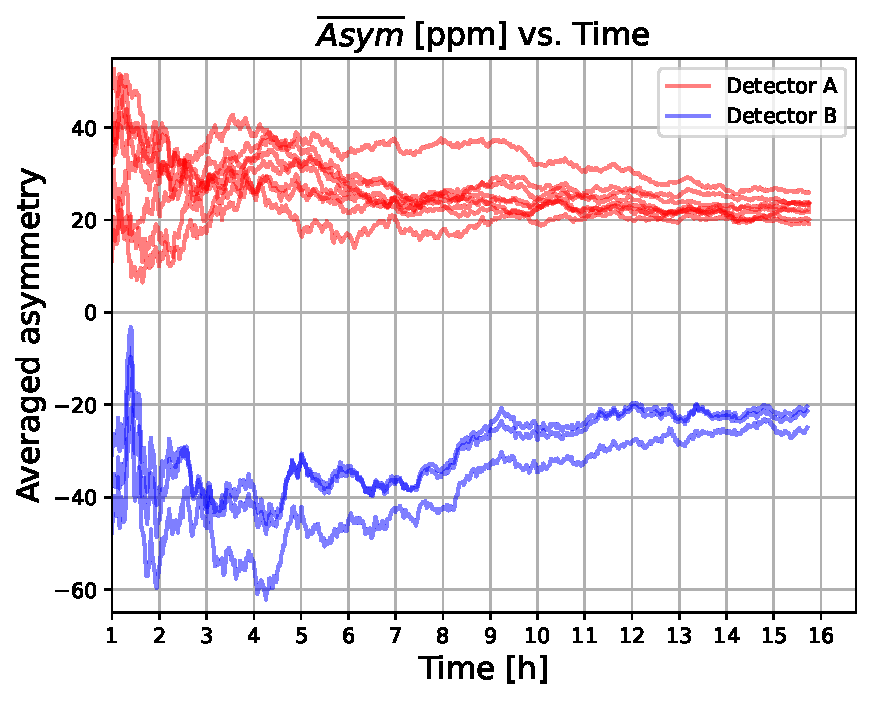
\includegraphics[width = 0.70\textwidth]{figures/AveragedAsymmetry.pdf}
\end{figure}
\end{frame}

\begin{frame}[noframenumbering]{Voltage to Frequency Converters}
The beam monitors are read-out with the voltage-to-frequency converters \textbf{VFC} devices, which produces an output signal whose frequency is proportional to the amplitude of the beam monitor signals. 
\begin{figure}
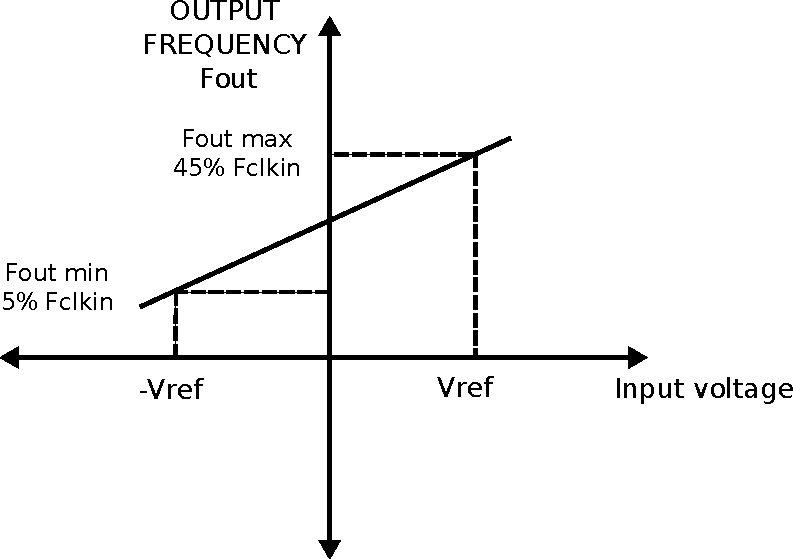
\includegraphics[width = 0.75\textwidth]{figures/Vfc.pdf}
\end{figure}
\end{frame}

% 9 DESCRIZIONE DEL PROCESSO
\begin{frame}[noframenumbering]{Description of the Process}

The transverse asymmetry arises considering the time reversal operator. The time reversal operator reverses all the momenta and the spin direction.

\begin{figure}[hbtp]
\centering
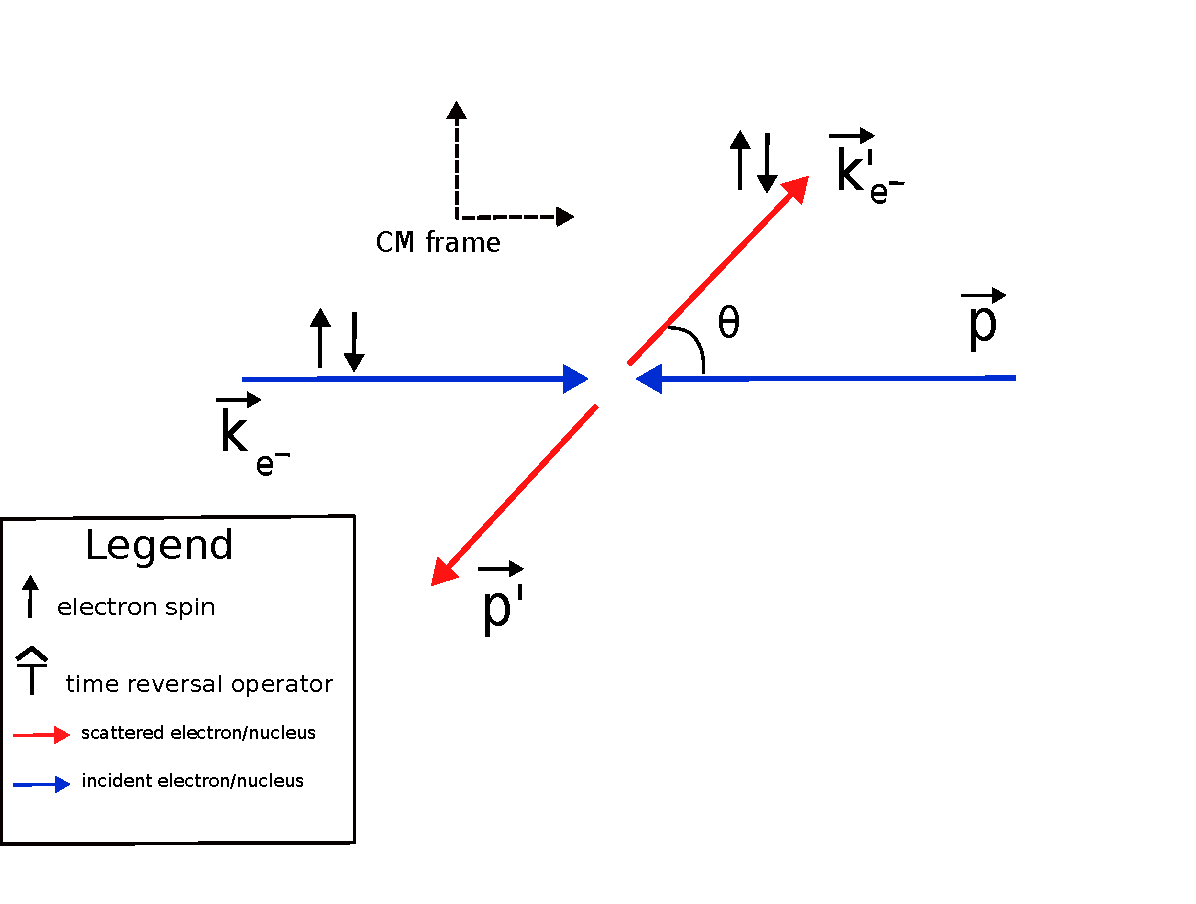
\includegraphics[width = 0.8\textwidth]{figures/ScatteringScheme.pdf}
\end{figure}

\end{frame}

\end{document}